% Options for packages loaded elsewhere
\PassOptionsToPackage{unicode}{hyperref}
\PassOptionsToPackage{hyphens}{url}
\PassOptionsToPackage{dvipsnames,svgnames,x11names}{xcolor}
%
\documentclass[
  letterpaper,
  DIV=11,
  numbers=noendperiod]{scrreprt}

\usepackage{amsmath,amssymb}
\usepackage{iftex}
\ifPDFTeX
  \usepackage[T1]{fontenc}
  \usepackage[utf8]{inputenc}
  \usepackage{textcomp} % provide euro and other symbols
\else % if luatex or xetex
  \usepackage{unicode-math}
  \defaultfontfeatures{Scale=MatchLowercase}
  \defaultfontfeatures[\rmfamily]{Ligatures=TeX,Scale=1}
\fi
\usepackage{lmodern}
\ifPDFTeX\else  
    % xetex/luatex font selection
\fi
% Use upquote if available, for straight quotes in verbatim environments
\IfFileExists{upquote.sty}{\usepackage{upquote}}{}
\IfFileExists{microtype.sty}{% use microtype if available
  \usepackage[]{microtype}
  \UseMicrotypeSet[protrusion]{basicmath} % disable protrusion for tt fonts
}{}
\makeatletter
\@ifundefined{KOMAClassName}{% if non-KOMA class
  \IfFileExists{parskip.sty}{%
    \usepackage{parskip}
  }{% else
    \setlength{\parindent}{0pt}
    \setlength{\parskip}{6pt plus 2pt minus 1pt}}
}{% if KOMA class
  \KOMAoptions{parskip=half}}
\makeatother
\usepackage{xcolor}
\setlength{\emergencystretch}{3em} % prevent overfull lines
\setcounter{secnumdepth}{5}
% Make \paragraph and \subparagraph free-standing
\makeatletter
\ifx\paragraph\undefined\else
  \let\oldparagraph\paragraph
  \renewcommand{\paragraph}{
    \@ifstar
      \xxxParagraphStar
      \xxxParagraphNoStar
  }
  \newcommand{\xxxParagraphStar}[1]{\oldparagraph*{#1}\mbox{}}
  \newcommand{\xxxParagraphNoStar}[1]{\oldparagraph{#1}\mbox{}}
\fi
\ifx\subparagraph\undefined\else
  \let\oldsubparagraph\subparagraph
  \renewcommand{\subparagraph}{
    \@ifstar
      \xxxSubParagraphStar
      \xxxSubParagraphNoStar
  }
  \newcommand{\xxxSubParagraphStar}[1]{\oldsubparagraph*{#1}\mbox{}}
  \newcommand{\xxxSubParagraphNoStar}[1]{\oldsubparagraph{#1}\mbox{}}
\fi
\makeatother

\usepackage{color}
\usepackage{fancyvrb}
\newcommand{\VerbBar}{|}
\newcommand{\VERB}{\Verb[commandchars=\\\{\}]}
\DefineVerbatimEnvironment{Highlighting}{Verbatim}{commandchars=\\\{\}}
% Add ',fontsize=\small' for more characters per line
\usepackage{framed}
\definecolor{shadecolor}{RGB}{241,243,245}
\newenvironment{Shaded}{\begin{snugshade}}{\end{snugshade}}
\newcommand{\AlertTok}[1]{\textcolor[rgb]{0.68,0.00,0.00}{#1}}
\newcommand{\AnnotationTok}[1]{\textcolor[rgb]{0.37,0.37,0.37}{#1}}
\newcommand{\AttributeTok}[1]{\textcolor[rgb]{0.40,0.45,0.13}{#1}}
\newcommand{\BaseNTok}[1]{\textcolor[rgb]{0.68,0.00,0.00}{#1}}
\newcommand{\BuiltInTok}[1]{\textcolor[rgb]{0.00,0.23,0.31}{#1}}
\newcommand{\CharTok}[1]{\textcolor[rgb]{0.13,0.47,0.30}{#1}}
\newcommand{\CommentTok}[1]{\textcolor[rgb]{0.37,0.37,0.37}{#1}}
\newcommand{\CommentVarTok}[1]{\textcolor[rgb]{0.37,0.37,0.37}{\textit{#1}}}
\newcommand{\ConstantTok}[1]{\textcolor[rgb]{0.56,0.35,0.01}{#1}}
\newcommand{\ControlFlowTok}[1]{\textcolor[rgb]{0.00,0.23,0.31}{\textbf{#1}}}
\newcommand{\DataTypeTok}[1]{\textcolor[rgb]{0.68,0.00,0.00}{#1}}
\newcommand{\DecValTok}[1]{\textcolor[rgb]{0.68,0.00,0.00}{#1}}
\newcommand{\DocumentationTok}[1]{\textcolor[rgb]{0.37,0.37,0.37}{\textit{#1}}}
\newcommand{\ErrorTok}[1]{\textcolor[rgb]{0.68,0.00,0.00}{#1}}
\newcommand{\ExtensionTok}[1]{\textcolor[rgb]{0.00,0.23,0.31}{#1}}
\newcommand{\FloatTok}[1]{\textcolor[rgb]{0.68,0.00,0.00}{#1}}
\newcommand{\FunctionTok}[1]{\textcolor[rgb]{0.28,0.35,0.67}{#1}}
\newcommand{\ImportTok}[1]{\textcolor[rgb]{0.00,0.46,0.62}{#1}}
\newcommand{\InformationTok}[1]{\textcolor[rgb]{0.37,0.37,0.37}{#1}}
\newcommand{\KeywordTok}[1]{\textcolor[rgb]{0.00,0.23,0.31}{\textbf{#1}}}
\newcommand{\NormalTok}[1]{\textcolor[rgb]{0.00,0.23,0.31}{#1}}
\newcommand{\OperatorTok}[1]{\textcolor[rgb]{0.37,0.37,0.37}{#1}}
\newcommand{\OtherTok}[1]{\textcolor[rgb]{0.00,0.23,0.31}{#1}}
\newcommand{\PreprocessorTok}[1]{\textcolor[rgb]{0.68,0.00,0.00}{#1}}
\newcommand{\RegionMarkerTok}[1]{\textcolor[rgb]{0.00,0.23,0.31}{#1}}
\newcommand{\SpecialCharTok}[1]{\textcolor[rgb]{0.37,0.37,0.37}{#1}}
\newcommand{\SpecialStringTok}[1]{\textcolor[rgb]{0.13,0.47,0.30}{#1}}
\newcommand{\StringTok}[1]{\textcolor[rgb]{0.13,0.47,0.30}{#1}}
\newcommand{\VariableTok}[1]{\textcolor[rgb]{0.07,0.07,0.07}{#1}}
\newcommand{\VerbatimStringTok}[1]{\textcolor[rgb]{0.13,0.47,0.30}{#1}}
\newcommand{\WarningTok}[1]{\textcolor[rgb]{0.37,0.37,0.37}{\textit{#1}}}

\providecommand{\tightlist}{%
  \setlength{\itemsep}{0pt}\setlength{\parskip}{0pt}}\usepackage{longtable,booktabs,array}
\usepackage{calc} % for calculating minipage widths
% Correct order of tables after \paragraph or \subparagraph
\usepackage{etoolbox}
\makeatletter
\patchcmd\longtable{\par}{\if@noskipsec\mbox{}\fi\par}{}{}
\makeatother
% Allow footnotes in longtable head/foot
\IfFileExists{footnotehyper.sty}{\usepackage{footnotehyper}}{\usepackage{footnote}}
\makesavenoteenv{longtable}
\usepackage{graphicx}
\makeatletter
\newsavebox\pandoc@box
\newcommand*\pandocbounded[1]{% scales image to fit in text height/width
  \sbox\pandoc@box{#1}%
  \Gscale@div\@tempa{\textheight}{\dimexpr\ht\pandoc@box+\dp\pandoc@box\relax}%
  \Gscale@div\@tempb{\linewidth}{\wd\pandoc@box}%
  \ifdim\@tempb\p@<\@tempa\p@\let\@tempa\@tempb\fi% select the smaller of both
  \ifdim\@tempa\p@<\p@\scalebox{\@tempa}{\usebox\pandoc@box}%
  \else\usebox{\pandoc@box}%
  \fi%
}
% Set default figure placement to htbp
\def\fps@figure{htbp}
\makeatother
% definitions for citeproc citations
\NewDocumentCommand\citeproctext{}{}
\NewDocumentCommand\citeproc{mm}{%
  \begingroup\def\citeproctext{#2}\cite{#1}\endgroup}
\makeatletter
 % allow citations to break across lines
 \let\@cite@ofmt\@firstofone
 % avoid brackets around text for \cite:
 \def\@biblabel#1{}
 \def\@cite#1#2{{#1\if@tempswa , #2\fi}}
\makeatother
\newlength{\cslhangindent}
\setlength{\cslhangindent}{1.5em}
\newlength{\csllabelwidth}
\setlength{\csllabelwidth}{3em}
\newenvironment{CSLReferences}[2] % #1 hanging-indent, #2 entry-spacing
 {\begin{list}{}{%
  \setlength{\itemindent}{0pt}
  \setlength{\leftmargin}{0pt}
  \setlength{\parsep}{0pt}
  % turn on hanging indent if param 1 is 1
  \ifodd #1
   \setlength{\leftmargin}{\cslhangindent}
   \setlength{\itemindent}{-1\cslhangindent}
  \fi
  % set entry spacing
  \setlength{\itemsep}{#2\baselineskip}}}
 {\end{list}}
\usepackage{calc}
\newcommand{\CSLBlock}[1]{\hfill\break\parbox[t]{\linewidth}{\strut\ignorespaces#1\strut}}
\newcommand{\CSLLeftMargin}[1]{\parbox[t]{\csllabelwidth}{\strut#1\strut}}
\newcommand{\CSLRightInline}[1]{\parbox[t]{\linewidth - \csllabelwidth}{\strut#1\strut}}
\newcommand{\CSLIndent}[1]{\hspace{\cslhangindent}#1}

\KOMAoption{captions}{tableheading}
\makeatletter
\@ifpackageloaded{bookmark}{}{\usepackage{bookmark}}
\makeatother
\makeatletter
\@ifpackageloaded{caption}{}{\usepackage{caption}}
\AtBeginDocument{%
\ifdefined\contentsname
  \renewcommand*\contentsname{Contenido}
\else
  \newcommand\contentsname{Contenido}
\fi
\ifdefined\listfigurename
  \renewcommand*\listfigurename{Lista de figuras}
\else
  \newcommand\listfigurename{Lista de figuras}
\fi
\ifdefined\listtablename
  \renewcommand*\listtablename{Lista de tablas}
\else
  \newcommand\listtablename{Lista de tablas}
\fi
\ifdefined\figurename
  \renewcommand*\figurename{Figura}
\else
  \newcommand\figurename{Figura}
\fi
\ifdefined\tablename
  \renewcommand*\tablename{Tabla}
\else
  \newcommand\tablename{Tabla}
\fi
}
\@ifpackageloaded{float}{}{\usepackage{float}}
\floatstyle{ruled}
\@ifundefined{c@chapter}{\newfloat{codelisting}{h}{lop}}{\newfloat{codelisting}{h}{lop}[chapter]}
\floatname{codelisting}{Listado}
\newcommand*\listoflistings{\listof{codelisting}{Lista de listados}}
\makeatother
\makeatletter
\makeatother
\makeatletter
\@ifpackageloaded{caption}{}{\usepackage{caption}}
\@ifpackageloaded{subcaption}{}{\usepackage{subcaption}}
\makeatother

\usepackage{bookmark}

\IfFileExists{xurl.sty}{\usepackage{xurl}}{} % add URL line breaks if available
\urlstyle{same} % disable monospaced font for URLs
\hypersetup{
  pdftitle={Manual de introducción a R},
  pdfauthor={Creado por: Dr.~Leonel Lerebours y Dr.~Yunior Rosario  Editado por: Lic. Virginia Vallejo},
  colorlinks=true,
  linkcolor={blue},
  filecolor={Maroon},
  citecolor={Blue},
  urlcolor={Blue},
  pdfcreator={LaTeX via pandoc}}


\title{Manual de introducción a R}
\author{Creado por: Dr.~Leonel Lerebours y Dr.~Yunior Rosario Editado
por: Lic. Virginia Vallejo}
\date{2025-07-29}

\begin{document}
\maketitle

\renewcommand*\contentsname{Contenido}
{
\hypersetup{linkcolor=}
\setcounter{tocdepth}{2}
\tableofcontents
}

\bookmarksetup{startatroot}

\chapter{Introducción}\label{introducciuxf3n}

\begin{center}\rule{0.5\linewidth}{0.5pt}\end{center}

\begin{center}\rule{0.5\linewidth}{0.5pt}\end{center}

\subsection{Consideraciones y recomendaciones de como mejorar el
autoaprendizaje en R (¡y en otra herramienta
similar!)}\label{consideraciones-y-recomendaciones-de-como-mejorar-el-autoaprendizaje-en-r-y-en-otra-herramienta-similar}

Este manual es muy específico para el entrenamiento de análisis de datos
en salud, tanto para el nivel básico como intermedio, y tiene como
propósito introducir el uso de R para ayudarte a facilitar el proceso de
desarrollo de tus productos de investigación. Con esto dicho, hay temas
que bien pudieran estar contenidos en un documento como este, pero por
lo específicos que son, no aparecen detallados en este manual; por
ejemplo, no abordaremos conceptos estadísticos básicos como las medidas
de tendencia central, por tanto, partimos del supuesto de que ya tienes
cierta familiaridad con estos temas. El enfoque principal es que puedas
comenzar a usar R, primero adaptándote al formato de comandos en vez del
formato orientado a objetos, (que es la manera como aprendiste Excel o
SPSS) y luego haciendo las tareas más comunes que se realizan
rutinariamente tanto en el entrenamiento como en la práctica, es decir,
hacer tablas, gráficos, exportar reportes, etc.; todo esto a un nivel
introductorio. El mundo de R es bien grande, (¡y qué bueno que es así!)
y al principio pudiera ser tedioso para ti aprender a usarlo, sin
embargo, desde que se comiences a producir resultados, notarás lo rápido
que avanzarás. Una de las razones por las que R es una solución muy
robusta para el análisis de grandes volúmenes de datos y para la
elaboración de reportes, es que hay una comunidad muy vasta de personas
que van aportando sus conocimientos y experiencia para hacer más fácil
el aprendizaje y el uso de R. En nuestros inicios, antes de ser
instructores, fueron muchos intentos de ensayo y error, es decir, era
agotador buscar en la web, ``googlear'' operaciones bien básicas del
tipo ``Cómo importar una base de datos de Excel a R'', o ``Como hacer
una tabla 2x2 en R'', o ``Cómo calcular la diferencia en días de una
misma columna de una variable fecha en un dataframe'' (esta última en
Excel es bien fácil, pero cuando hay que hacerlo con una base de datos
bien grande, Excel colapsa mientras que con R es más rápido); otra tarea
de apoyo en nuestros inicios era leer tutoriales, aplicarlos, obtener
resultados erróneos, corregir, preguntar\ldots{} en fin, dar muchas
vueltas hasta dar con lo que andábamos buscando. Este tipo de esfuerzos
en la actualidad es muy diferente actualmente debido al uso de la
inteligencia artificial como una plataforma que provee facilidades para
avanzar rápido con el aprendizaje de cualquier lenguaje informático. Lo
que ha sido un común denominador es que siempre hay respuestas, y
muchas, de cómo hacerlo de diferentes formas, cualquier cosa
(¡Relacionada al análisis de datos!). En pocas palabras, cualquier
problema o tarea que quieras hacer en R es muy probable que ya alguien
la haya hecho. Este manual es un ejemplo de eso, pues aprendimos a usar
este lenguaje que literalmente es difícil, sin embargo, lo hemos
simplificado para ti, ayudándote a reducir considerablemente el tiempo
de búsqueda en tutoriales y Chat GPT, combinando el lenguaje de R y el
lenguaje clínico. Lo más interesante de aprender a usar R con este
estilo de ensayo y error es que aprendimos cosas que no teníamos la
menor idea de que existían, por ejemplo, la teoría de los colores, la
gramática de los gráficos, ejercicios estadísticos que pensábamos eran
imposibles hacer en R, sin embargo, por la cantidad de tutoriales,
ayudas, videos, cursos (la gran mayoría gratuitos o de muy bajo costo),
hemos tenido la oportunidad de aprender más allá de lo esperado y te lo
traemos resumido y bajo una metodología práctica, para que puedas
aplicarlo de inmediato en tus tareas cotidianas. De una forma u otra, el
mundo de R representa un gran avance donde converge la tecnología y la
buena voluntad de muchas personas, sin fines de lucro, que realmente
creen en el crecimiento social a través de la información; por
herramientas como R se ha popularizado el uso de la ciencia de datos,
que es muy usada en muchas profesiones incluyendo la epidemiología, y ha
facilitado mucho el proceso de difundir información, como las
publicaciones de artículos. Entonces, como parte de la experiencia de
comenzar a usar R es el autoaprendizaje, te invitamos como primera tarea
o ejercicio a que ``busques'' qué es R, quiénes lo crearon, para qué lo
crearon, y haciendo esta actividad te vas a dar cuenta lo mencionado en
las líneas anteriores sobre la vasta cantidad de información disponible
en cuanto al uso de R para la gestión de datos. Por último, el
ingrediente principal para aprender este lenguaje es tener en qué
usarlo, es decir, una necesidad, en este caso, sobre procesamiento,
análisis y reporte de datos. Esperamos que te motives a implementar esta
herramienta y que te sea de provecho este manual, para que puedas seguir
aprendiendo más de lo que esperas aprender durante este curso.

\subsection{Definiciones claves}\label{definiciones-claves}

\begin{itemize}
\item
  \textbf{Objetos:} Son elementos que almacenan información y pueden ser
  de diferentes tipos como un valor simple (numérico o caracter), un
  dataframe, un vector, una función, una lista, gráficos entre otros. De
  forma abstracta un objeto es un contenedor que puede almacenar uno o
  varios elementos. Estos se ``almacenan'' en el ambiente de trabajo que
  reside en la memoria de la PC. Los objetos se crean usando el operador
  de asignación ``\textbf{\textless-}'' o signo ``=''.
\item
  \textbf{Dataframe:} Es el equivalente a una base de datos en formato
  de tabla o listado, donde cada columna es una variable y cada fila es
  una observación.
\item
  \textbf{Vector:} Un vector es un objeto que consiste una lista de
  elementos que son del mismo tipo.
\item
  \textbf{Rutina:} Es un conjunto de comandos o códigos que cumplen con
  una tarea en específico, ejemplo la importación de una base de datos y
  su limpieza (en inglés se le dice \emph{script})
\item
  \textbf{Paquete:} Son varios archivos que contienen funciones,
  documentación, bases de datos. Son fundamentales para añadir
  funcionalidad a R. También es la vía como se comparte códigos
  re-producibles (funciones). A modo de analogía un paquete vendría
  siendo una herramienta (destornillador, martillo) y R sería la mesa de
  trabajo, donde cada vez que necesitas una herramienta (paquete) la
  traes a la mesa de trabajo.
\item
  \textbf{Proyecto:} ``Un proyecto es una carpeta de trabajo designado
  con un archivo .RProj. Al abrir un proyecto (usando Archivo
  -\textgreater{} Abrir proyecto en RStudio o haciendo doble clic en el
  archivo .Rproj fuera de R), la carpeta de trabajo se establecerá
  automáticamente en el directorio donde se encuentra el archivo .RProj.
\item
  \textbf{Bases de datos} en diferentes formatos, preferiblemente en
  .csv, pero en Excel u otros formatos comunes se pueden trabajar)
\item
  \textbf{Operadores :} Según en el libro de R para principiantes de
  Juan Bosco Mendoza (\textbf{vega?}): \emph{``Son los símbolos que le
  indican a R que debe realizar una tarea. Combinando datos y operadores
  es que logramos que R haga su trabajo. Existen operadores específicos
  para cada tipo de tarea. Los tipos de operadores principales son los
  siguientes: Aritméticos, Relacionales, Lógicos y De asignación.''}
\item
  \textbf{Expresión:} En programación, una expresión es una combinación
  de constantes, variables o funciones, que es interpretada de acuerdo a
  las normas particulares de precedencia y asociación para un lenguaje
  de programación en particular.
\item
  \textbf{Código:} son los signos y símbolos que tienen un significado o
  en sus diferentes combinaciones se pueden interpretar como un lenguaje
\item
  \textbf{Función:} es un bloque de código reutilizable que realiza una
  tarea específica, tomando argumentos como entrada y devolviendo un
  resultado, lo que facilita la organización y reutilización del código.
\item
  \textbf{Argumento:} es un valor o variable que se pasa a una función
  para que la función pueda realizar su tarea específica
\item
  \textbf{Variable:} es un nombre que se le asigna a un valor o objeto,
  que puede ser de diferentes tipos (números, texto, etc.) y que se
  almacena en la memoria de la computadora.
\end{itemize}

\bookmarksetup{startatroot}

\chapter{Preparación del ambiente de
trabajo}\label{preparaciuxf3n-del-ambiente-de-trabajo}

\section{Como se instala R y
Rstudio®}\label{como-se-instala-r-y-rstudio}

El primer paso para esta tarea es descargar el programa R, que se
encuentra en la página web \url{https://cran.r-project.org/} . en esta
hay varias versiones dependiendo que sistema operativo estás usando, ya
sea Windows, macOS o Linux.

\begin{figure}[H]

{\centering \pandocbounded{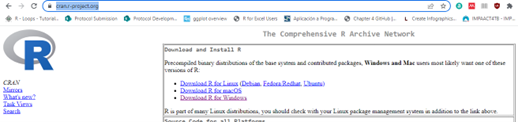
\includegraphics[keepaspectratio]{imagenes/01rwebpage.png}}

}

\caption{En esta página trata de descargar la versión más actualizada}

\end{figure}%

Luego de descargarlo puedes instalarlo inmediatamente usando el
ejecutable (para Windows y macOS) o la forma como se instalan software
in Linux. Para este manual estamos en un ambiente de Windows, luego de
instalar podemos acceder a la \textbf{\emph{consola}} de R (una pantalla
con un cursor parpadeando donde podemos escribir)

\begin{figure}[H]

{\centering \pandocbounded{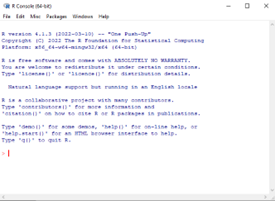
\includegraphics[keepaspectratio]{imagenes/01consolar.png}}

}

\caption{Este es la consola de R, aquí podemos comenzar a usar R, pero
es un poco complejo usar solamente la consola}

\end{figure}%

Aunque ya hayamos instalado R, al menos que seamos muy expertos en su
uso, que conozcamos bien las sintaxis de las funciones, que
\textbf{\emph{objetos}} (más tarde veremos lo que son los objetos) están
cargados en la memoria, entre otras cosas (¡también se puede usar como
una simple calculadora!), es muy complicado usar solamente la consola,
por lo que tenemos disponible aditamentos o accesorios que nos permiten
trabajar más fácil con R, así como su aprendizaje. Para este manual el
aditamento que usaremos es \textbf{Rstudio} de
\href{https://posit.co/}{Posit®}.

\subsection{Descargar e instalar
Rstudio}\label{descargar-e-instalar-rstudio}

Ahora vamos a instalar Rstudio, para esto vamos a descargarlo de la
siguiente página web,
\href{https://posit.co/download/rstudio-desktop/}{Descarga de Rstudio}
donde vamos a buscar la versión gratuita de escritorio para para el
sistema operativo que estamos usando.

En caso de que estés usando Linux, están las instrucciones en la página
de como hacerlo, la versión de Windows y macOS es un ejecutable.

Luego de descargar la ultima versión disponible procedemos a instalar
Rstudio, haciendo clic en el ejecutable, la instalación (en la versión
de Windows por ejemplo) es muy similar a cualquier otro software que
donde te pregunta el lugar donde será instalado y varias ventanas donde
se ve el progreso de instalación. Si todo salió bien, es decir que se
instaló sin errores, pues tendremos disponible en la barra de acceso
directo y en el escritorio, (si elegimos esta opción durante la
instalación) también tendremos un acceso directo.

Si tienes Windows, te compartimos el paso a paso en
\href{https://1drv.ms/v/c/e5de2b13338e6a60/ERlqk9CSPdpLs58edQq_s4kB_mIE4vURE-BxuRT3p6K-8Q?e=BNB7q9}{este
video} para descargar e instalar R y también R Studio Desktop.

\begin{figure}[H]

{\centering \pandocbounded{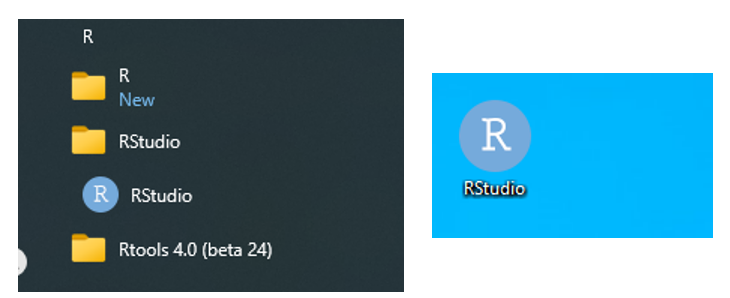
\includegraphics[keepaspectratio]{imagenes/01conorstudio.png}}

}

\caption{En Windows, la barra de inicio o las aplicaciones y si se creó
el acceso directo (derecha) en el escritorio}

\end{figure}%

Otro software que se debe instalar si el sistema operativo que usas es
Windows es \textbf{rtools}, dado que algunos paquetes necesitan que esté
instalado para funcionar de forma correcta.

Este se adquiere desde la página de
\href{https://cran.r-project.org/bin/windows/Rtools/}{Descarga rtools} y
elige la versión más reciente y descarga el formato ejecutable (termina
en ``installer'') en cualquier unidad de almacenamiento. Su instalación
sencilla, solo ejecutar el programa y hacer clic en siguiente las veces
que sea necesario.

\begin{figure}[H]

{\centering \pandocbounded{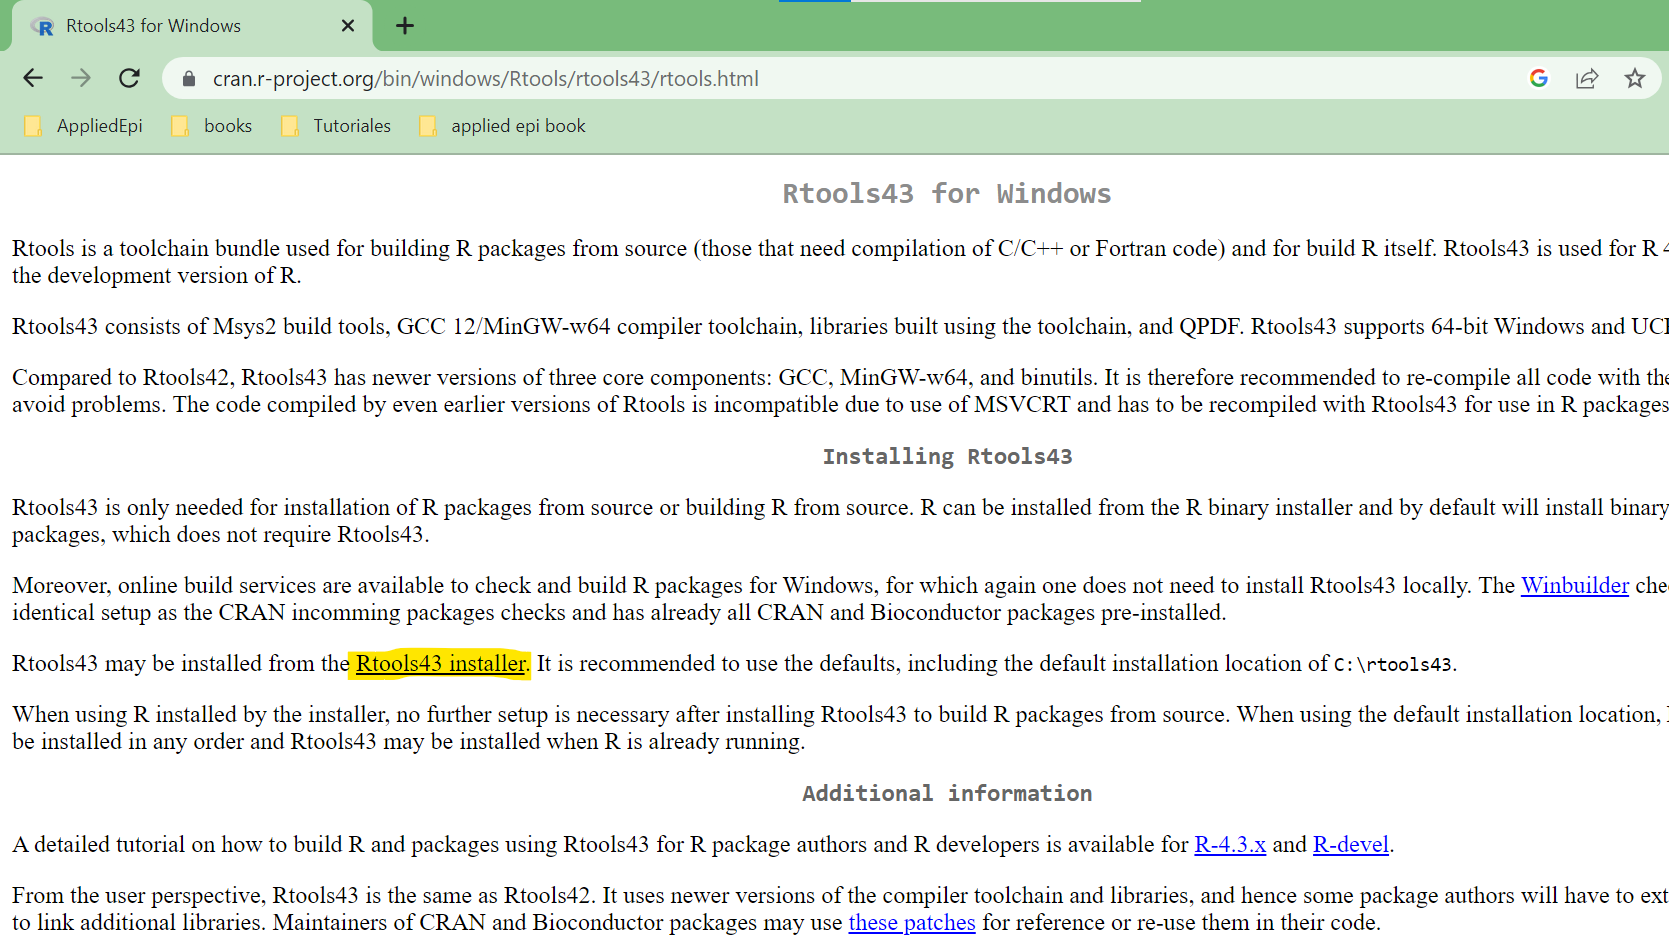
\includegraphics[keepaspectratio]{imagenes/01rtools.png}}

}

\caption{Busca esta version señalada en la imagen}

\end{figure}%

\section{Interfaz de Rstudio®}\label{interfaz-de-rstudio}

Para facilitar el aprendizaje y uso de R, vamos a usar RStudio que es un
entorno de desarrollo integrado o IDE (Integrated Development
Environment) y tiene la gran ventaja de que hay mucha documentación
sobre su uso, es muy cómoda de trabajar porque nos ayuda con la
escritura de los códigos, la organización de los archivos, tiene varios
visores o paneles para ver los códigos, las salidas, los objetos
cargados y otras ayudas más (Figura 5). RStudio ha permitido la difusión
del uso de R, lo que ha permitido la propagación de su uso en todas las
áreas donde se hace análisis de datos.

\begin{figure}[H]

{\centering 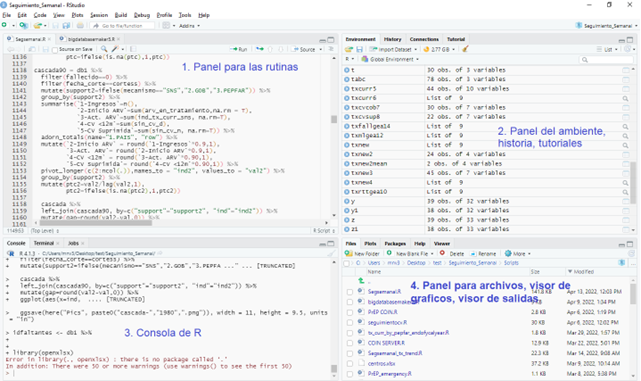
\includegraphics[width=6.6875in,height=\textheight,keepaspectratio]{imagenes/01interfazrstudio.png}

}

\caption{En esta imagen podemos ver los 4 paneles principales y el menú
de la interfaz de Rstudio}

\end{figure}%

\begin{enumerate}
\def\labelenumi{\arabic{enumi}.}
\item
  \textbf{Panel de las rutinas:}~este panel es el editor de texto donde
  vamos a escribir los códigos (rutinas) que vamos a usar para nuestras
  tareas, como las tablas, los gráficos, etc., que son automáticamente
  ejecutadas en la consola de R. Cada rutina se puede guardar como un
  archivo (muy similar a un archivo de texto normal), la característica
  más importante de este panel es que nos permite ver si el código tiene
  errores, pues a veces la falta de una simple coma o un caracter nos
  arroja error cuando ejecutamos comandos. También nos ofrece la
  herramienta de autocompletar y nos facilita mucho la organización del
  código. Para ejecutar una línea de código simplemente ponemos el
  cursor al inicio o al final de la línea y presionamos Ctrl+Enter o en
  el botón ``run'', mientras que para ejecutar la rutina completa,
  hacemos clic en el botón ``source''. Más adelante veremos varios
  ejemplos.
\item
  \textbf{Panel del ambiente} de trabajo \textbf{o panel de objetos
  cargados:} en este panel podemos ver cuales objetos tenemos cargados
  en la memoria del sistema, y nos permite ver qué tipo de objeto es (si
  es un \emph{dataframe}, un \emph{vector}, una \emph{matriz}, una
  \emph{función}, una l\emph{ista}). Esto nos ayuda a seguir el trabajo
  que vamos realizando, por ejemplo, cuando cargamos una base de datos
  desde un archivo de Excel en un objeto \emph{dataframe} podemos ver
  cuantas filas y variables tiene el archivo. También a través de este
  panel podemos salvar la sesión de trabajo, esto es útil cuando hacemos
  una pausa y queremos retomar más adelante lo que estábamos haciendo.
\item
  \textbf{Consola de R:} este es el lugar donde ocurre todo, puedes
  directamente escribir los comandos, las funciones, etc., pero para
  esto tenemos el panel de las rutinas, aquí también vas a ver los
  mensajes de errores cuando ejecutas una rutina o un comando, y por
  cada línea que se escribe se presiona ``enter'' para ejecutar los
  comandos. La ventaja más grande de utilizar RStudio es que hasta en la
  consola te identifica si hay errores o comandos incompletos y
  autocompletar.
\item
  \textbf{Panel para archivos, visor de gráficos y de salidas:} en este
  panel tenemos varias ventanas donde nos permite ver los archivos
  disponibles (muy parecido al explorador de Windows o a la carpeta de
  Documentos de tu computadora). A través del menú de este panel podemos
  crear carpetas, borrar, mover o copiar archivos, también podemos
  definir el directorio de trabajo (vamos a ver más adelante en detalle
  qué es el directorio o lugar de trabajo), a la derecha de Archivos o
  Files está el visor de gráficos (Plots), que podemos ampliar y poder
  copiar el gráfico que se está presentando y más a la derecha está el
  visor de salidas (Viewer), como tablas y datos en formato HTML.
  También en este panel está la ventana para instalar paquetes (término
  muy importante que lo veremos más adelante) y la ventana de ayuda
  (Figura 6).

  \begin{figure}[H]

  {\centering 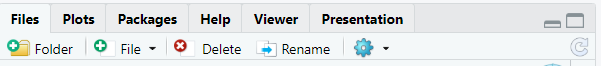
\includegraphics[width=5.32292in,height=\textheight,keepaspectratio]{imagenes/01figura06.png}

  }

  \caption{Figura 6.}

  \end{figure}%
\end{enumerate}

Antes de comenzar a trabajar puedes ir familiarizándote con esta
interface. En RStudio hay muchas opciones que iremos explicando en la
medida que vayamos avanzando, mientras tanto, te mostrados dos
herramientas interesantes del menú principal de RStudio: \textbf{Tools}
y \textbf{Help}.

Si vas al menú principal de RStudio, puedes entrar en la sección que
dice~\textbf{``Tools''} y dentro del menú desplegable seleccionas la
opción de \textbf{``Global Options''}~(al final del menú desplegable),
allí encontrarás un menú, y dentro de ``\textbf{Appearance}'' está la
opción ``Editor theme'' donde podrás cambiar los colores y el tipo de
letra de las ventanas, así podrás para adaptar el ambiente a tu gusto.
En Ayuda (Help) puedes encontrar los accesos directos para usar el
teclado, por ejemplo, salvar la rutina en la que estás trabajando,
reiniciar R, ejecutar toda la rutina, entre otros atajos. En la Figura 7
te mostramos cómo llegar a cada una de estas herramientas.

\begin{figure}[H]

{\centering 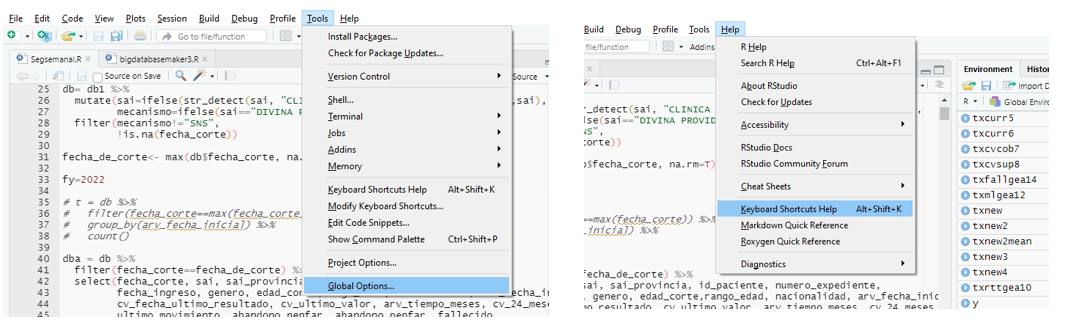
\includegraphics[width=8.48in,height=\textheight,keepaspectratio]{imagenes/01menurstudio.png}

}

\caption{Figura 7. Seleccionar ``Tool'' luego ``Global Options'' y en
ayuda, buscar los atajos del teclado}

\end{figure}%

\section{Instalación de Paquetes (librerías de
funciones)}\label{instalaciuxf3n-de-paquetes-libreruxedas-de-funciones}

Los paquetes son extensiones para añadir más funcionalidades a R. Es
quizás la razón por la cual R es ahora mismo una de las mejores
herramientas para trabajar con datos dada la cantidad de paquetes
específicos para realizar tareas como hacer tablas por ejemplo. En la
literatura, los paquetes se identifican con \{ \}, ejemplo:
\textbf{\{tidyverse\}} y los logos son una figura dentro de un hexágono.

Con respecto a la instalación de paquetes, usualmente estos deben estar
publicados en CRAN (\href{https://cran.r-project.org/web/packages/}{Aquí
el enlace}) y se instalan desde el panel de paquetes (``Packages'').

\pandocbounded{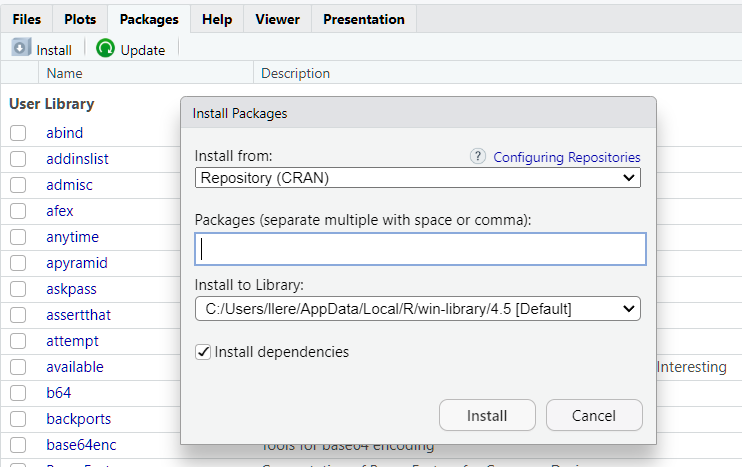
\includegraphics[keepaspectratio]{imagenes/01packages3.png}}

\section{Como instalar y cargar un paquete en
R}\label{como-instalar-y-cargar-un-paquete-en-r}

Después de instalar R, Rstudio solo tenemos las funcionalidades que trae
\textbf{R base}, que nos permiten hacer muchas cosas sin tener que
instalar nada más, pero podemos hacer que R sea más completo, ahora
vamos a ver que es un paquete y su importancia.

Como R es un lenguaje de programación por lo tanto podemos crear
programas o conjunto de funciones y estos programas podemos exportarlos
para luego usarlos más adelante.

Estos programas o complementos aumentan la capacidad de R a través de
funciones o comandos, por ejemplo, \textbf{R base}, no nos permite
exportar directamente los resultados o salidas en formato Excel o crear
tablas con formato de forma directa. Por lo tanto, los paquetes o
subprogramas hacen que R sea más que solo un lenguaje de programación.

Hay paquetes creados por epidemiólogos, para epidemiólogos como el
\textbf{epitools} (Tomas J. Aragon) (\textbf{aragon2020?}) o
\textbf{epikit} (Zhian N. Kamvar)(\textbf{spina2023?}) que nos permiten
con pocos comando o funciones hacer tareas como calcular medidas de
asociación (OR, Riesgo relativo) y facilitar los análisis en
epidemiología y otros paquetes que hacen las tareas de análisis de datos
como son el \textbf{openxlsx} (Philipp
Schauberger)(\textbf{schauberger2023?}) para manipular y crear archivos
de Excel o el muy famoso y aclamado paquete \textbf{tidyverse} (Hadley
Wickham)(\textbf{wickham2023?})del cual hay este paquete hay libros
escritos para el procesamiento y manejo de datos por mencionar algunos.

Los paquetes nos permiten mejorar sobremanera nuestra productividad en
general. Cada vez que iniciamos una sesión con Rstudio, en nuestras
rutinas debemos cargar los paquetes que vamos a usar.

Dado que R es una plataforma colaborativa, cuando un paquete es creado
pasa por un proceso de validación antes de ser publicados en el
repositorio de R. Es por esto que, para su instalación debemos saber si
están disponibles. Los paquetes, usualmente, después de ya ser
validados, son publicados en el repositorio de R (The Comprehensive R
Archive Network o \href{https://cran.r-project.org/web/packages/}{CRAN})
que es la página donde descargamos R. También pueden estar disponibles
en otras páginas donde podemos descargarlos e instalarlos manualmente.
Después de instalar un paquete solo es necesario verificar si ha sido
actualizado, tal como haces con cualquier otro programa.

Usualmente los autores de los paquetes tienen tutoriales o páginas
llamadas ``Vignettes'' o viñetas donde podemos ver las funcionalidades y
tutoriales. Por ejemplo, ejemplo ingresa en la barra de búsqueda en tu
explorador estas palabras: ``R package epitools'', y aparecerán muchos
resultados para diferentes tareas. Sigue estos pasos para verificar si
un paquete existe buscando directamente desde RStudio:

\begin{enumerate}
\def\labelenumi{\arabic{enumi}.}
\tightlist
\item
  Ir al panel de archivos
\item
  Hacer clic en la ventana de paquetes o ``Packages''
\item
  Hacer clic en ``install''. Aparecerá una ventana donde escribirás el
  nombre del paquete. Si el paquete existe en CRAN, aparecerá en un
  listado y lo seleccionarás
\item
  Hacer clic en ``install''.
\end{enumerate}

\begin{figure}[H]

{\centering \pandocbounded{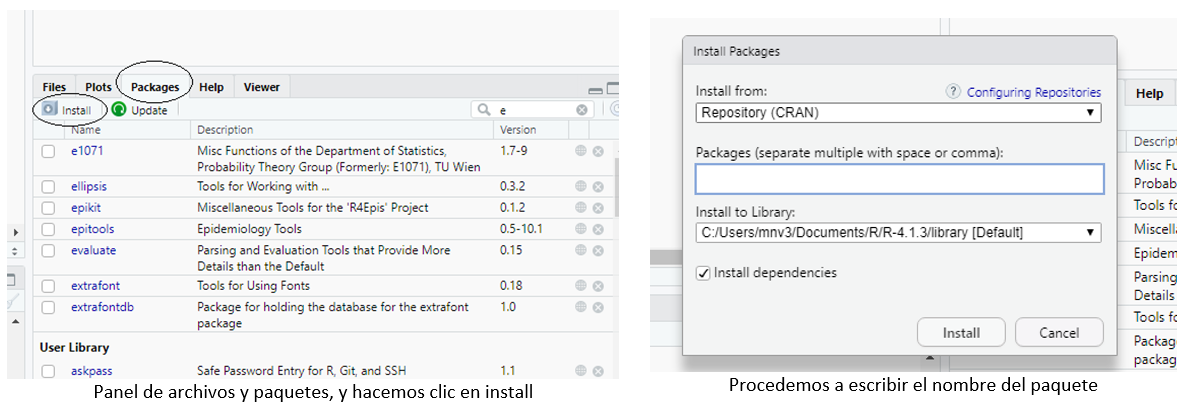
\includegraphics[keepaspectratio]{imagenes/01packages.png}}

}

\caption{installando un paquete en Rstudio}

\end{figure}%

Si el paquete no está disponible en CRAN pero si en la web y podemos
descargarlo y cambiar donde dice \textbf{``install from''} a
\textbf{``package archive file''} y buscar en el disco duro y proceder a
instalar (es muy raro que se de este caso y los paquetes que vamos a
instalar todos están disponible en CRAN).

La otra forma de instalar los paquetes es directamente desde la consola
o en un archivo de rutina usando el la función
\textbf{\emph{install.package()}} donde escribimos entre comillas el
nombre del paquete que queremos instalar.

\begin{figure}[H]

{\centering \pandocbounded{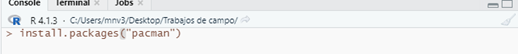
\includegraphics[keepaspectratio]{imagenes/01packages2.png}}

}

\caption{Figura 14. En esta imagen vemos en la consola la función para
instalar el paquete pacman}

\end{figure}%

Luego de esta introducción sobre qué es un paquete y cómo se instala,
vamos a hacer el siguiente ejercicio de instalar varios paquetes que
usaremos de forma constante en los ejercicios y tareas contenidos en
este manual. Ya sea directamente en la consola (ver imagen anterior), o
a través del panel de archivos, vamos a instalar este
paquete~\textbf{``pacman''}~(Tyler Rinker)~que es un paquete para
manejar paquetes y nos ahorrará muchos pasos, por ejemplo, detecta si un
paquete necesario está instalado o no, y procede a instalarlo, o ayuda a
instalar paquetes desde otras fuentes alternativas a CRAN. Después de
instalarlo podemos ver en la consola el mensaje de que se instaló
correctamente~ \textbf{(\emph{package `pacman' successfully unpacked and
MD5 sums checked}).}

En la rutina que comenzamos hace un momento atrás vamos a hacer la
siguiente tarea:

\begin{itemize}
\tightlist
\item
  Escribe o copia y pega el siguiente comando (recuerda, para ejecutar
  un comando o varios selecciona estos y presiona Ctrl+Enter o clic en
  ``Run''):
\end{itemize}

\begin{Shaded}
\begin{Highlighting}[]
\NormalTok{pacman}\SpecialCharTok{::}\FunctionTok{p\_load}\NormalTok{(}\StringTok{"tidyverse"}\NormalTok{, }\StringTok{"janitor"}\NormalTok{, }\StringTok{"gtsummary"}\NormalTok{, }\StringTok{"epikit"}\NormalTok{,}\StringTok{"here"}\NormalTok{,                }\StringTok{"epitools"}\NormalTok{, }\StringTok{"lubridate"}\NormalTok{, }\StringTok{"openxlsx"}\NormalTok{, }\StringTok{"readxl"}\NormalTok{, }\StringTok{"rio"}\NormalTok{)}
\end{Highlighting}
\end{Shaded}

Espera un momento si es la primera vez que se ejecuta para que así se
instalen los paquetes que están en el comando.. Antes de continuar,
vamos a explicar el comando anterior:

En Rstudio, en el editor de rutinas o en la misma consola, cuando
queremos ver las funciones o comandos disponibles en un paquete podemos
escribir el nombre del paquete seguido de dos puntos nos aparecerá una
ventana con un listado de dichas funciones, por ejemplo, este último
comando usamos el paquete \textbf{pacman} y dentro de este paquete
usamos la función de \textbf{\emph{p\_load}} (para cargar paquetes, que
también los instala si no están ya instalados)

\begin{figure}[H]

{\centering \pandocbounded{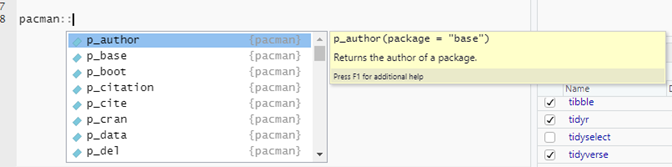
\includegraphics[keepaspectratio]{imagenes/01pacman.png}}

}

\caption{Esta es una de las funcionalidades de Rstudio que nos facilitan
el trabajo , luego de escribir el nombre del paquete y dos veces dos
puntos nos aparece el listado de funciones y también una ventana
amarilla para ayuda de la función presionando F1 para ver en el panel de
archivos, la ventana de ayuda y así ver los ejemplos de cómo usar dicha
función.}

\end{figure}%

Luego de escribir el nombre del paquete y dos veces dos puntos, nos
aparece el listado de funciones y también una ventana amarilla para
ayuda de la función, que también aparece presionando F1 o haciendo una
búsqueda en el panel de archivos en la ventana de ayuda, donde también
se pueden ver los ejemplos de cómo usar las funciones.

Los paquetes que hemos instalado hasta este momento no los vamos a
detallar por ahora, sino que, en la medida que vayamos haciendo los
ejercicios, vamos a ir explicando para qué sirven a través de las
funciones que traen cada uno. Es oportuno señalar que, dentro de los
paquetes disponibles en R, existen paquetes útiles para facilitar el
proceso de importar y exportar funciones específicas para las tareas del
epidemiólogo, para hacer reportes y para facilitar el proceso de la
gestión de los datos.

Para ver que paquetes tenemos cargados podemos escribir en la consola
\textbf{\emph{search()}}

\begin{Shaded}
\begin{Highlighting}[]
\FunctionTok{search}\NormalTok{()}
\end{Highlighting}
\end{Shaded}

\begin{verbatim}
 [1] ".GlobalEnv"        "package:rio"       "package:readxl"   
 [4] "package:openxlsx"  "package:epitools"  "package:here"     
 [7] "package:epikit"    "package:gtsummary" "package:janitor"  
[10] "package:lubridate" "package:forcats"   "package:stringr"  
[13] "package:dplyr"     "package:purrr"     "package:readr"    
[16] "package:tidyr"     "package:tibble"    "package:ggplot2"  
[19] "package:tidyverse" "package:stats"     "package:graphics" 
[22] "package:grDevices" "package:utils"     "package:datasets" 
[25] "package:methods"   "Autoloads"         "package:base"     
\end{verbatim}

Los dos capítulos siguientes son muy importantes. Debes familiarizarte
con ellos porque son los fundamentos para poder trabajar en R, veremos
ejemplos de las sintaxis de las expresiones, los diferentes tipos de
objetos de datos, y a medida que vayamos practicando se irá haciendo más
fácil entender el código, las funciones y las operaciones que hacemos.
Te recomendamos que, aparte de este manual, abundes más sobre los temas
que verás a continuación para que agilices tu proceso de aprendizaje con
R.

\bookmarksetup{startatroot}

\chapter{Comenzar a trabajar con R y la interfaz de
Rstudio}\label{comenzar-a-trabajar-con-r-y-la-interfaz-de-rstudio}

Ya luego de tener todo lo necesario instalado, ahora vamos a realizar
los siguientes pasos con la finalidad de ir aprendiendo a organizar los
trabajos que estaremos haciendo, como son los productos o asignaciones
que se deben hacer durante la capacitación, como son los análisis de
vigilancia, análisis de brotes, evaluación de sistema de vigilancia
entre otros.

Una gran recomendación es tener lo más organizado posible cada elemento
hecho en R o cualquier documento asociado a los análisis o trabajos que
vas a realizar; esto porque en nuestro caso, cuando comenzamos a
trabajar con RStudio guardábamos las rutinas y las salidas en diferentes
lugares, como principiantes al fin, no teníamos una estructura, y luego
cuando necesitábamos re-usar una rutina, buscar un documento de salida
era muy difícil de encontrar y perdíamos tiempo en esa búsqueda, a veces
nos tomaba más que lo que se toma ejecutar una rutina. Luego aprendimos
sobre lo que vamos a ver a continuación en cuanto a trabajar bajo
proyectos en RStudio.

\section{Creación de un proyecto}\label{creaciuxf3n-de-un-proyecto}

El primer paso para comenzar es decidir dónde estarán los archivos
relacionados al o a los trabajos que se van a hacer, es decir, debes
definir si almacenarás tu trabajo en un disco dentro de la PC o en la
``Nube'' (ejemplo, OneDrive, Google drive) para que así siempre
facilites tu trabajo, especialmente cuando necesites hacer cambios o
actualizar las bases de datos.

Esto es sumamente importante dado que nos ayudará a mantenernos
organizados. Todos los archivos como las bases de datos, las
referencias, las rutinas, deben estar almacenados en un lugar donde te
sea fácil encontrarlos y también para la ejecución o desarrollo del
proyecto o proyectos en que estés trabajando.

Para el segundo paso vamos a entrar en RStudio y vamos a crear un
\textbf{archivo de proyecto} de la siguiente forma:

\begin{figure}[H]

{\centering 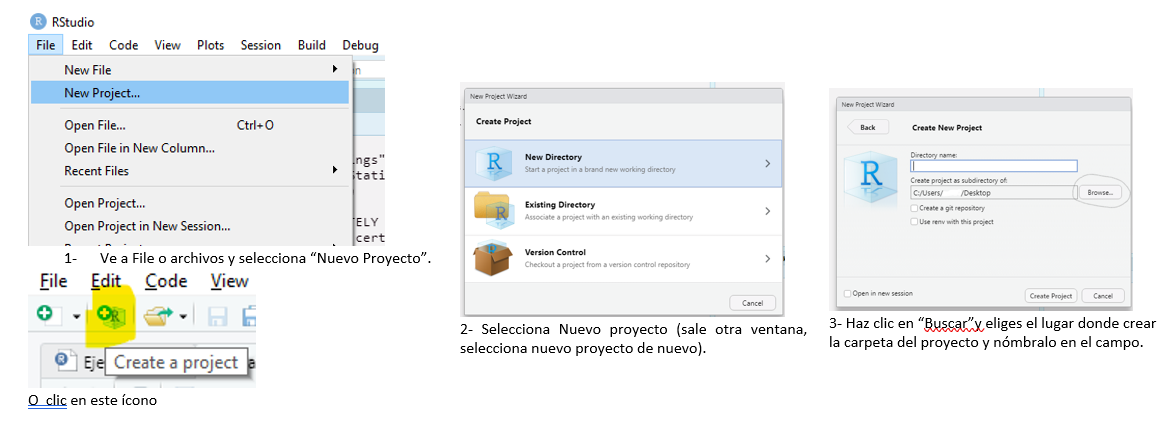
\includegraphics[width=6.18in,height=\textheight,keepaspectratio]{imagenes/01proyectonuevo.png}

}

\caption{Figura 10. Creando un proyecto}

\end{figure}%

\begin{enumerate}
\def\labelenumi{\arabic{enumi}.}
\item
  Crea el proyecto llamándolo ``mi\_primer\_proyecto'' siguiendo los
  pasos de la Figura 10.
\item
  Guarda el proyecto nuevo en el ``escritorio'' o en ``Documentos'' si
  usas Windows.
\item
  Para crear las carpetas, en la ventana inferior derecha o panel para
  archivos, ve a ``Archivos'' o ``File'', luego haz clic en ``new
  folder'' para crear las siguientes carpetas:
\end{enumerate}

\begin{enumerate}
\def\labelenumi{\alph{enumi}.}
\item
  ``Base de datos'' para almacenar tus datos en cualquier formato, como
  datos en Excel, por ejemplo.
\item
  ``Rutinas'' para salvar las rutinas que irás creando.
\item
  ``Referencias'' vas a poner aquí los documentos de soporte como
  referencias, artículos, etc.
\item
  ``Salidas'', donde vamos a salvar los documentos generados a partir de
  las rutinas, en esta última podemos tener una subcarpeta que se llame
  ``imágenes'' para las salidas que son imágenes, como gráficos o tablas
  salvadas en formato de imagen.
\end{enumerate}

\begin{figure}[H]

{\centering 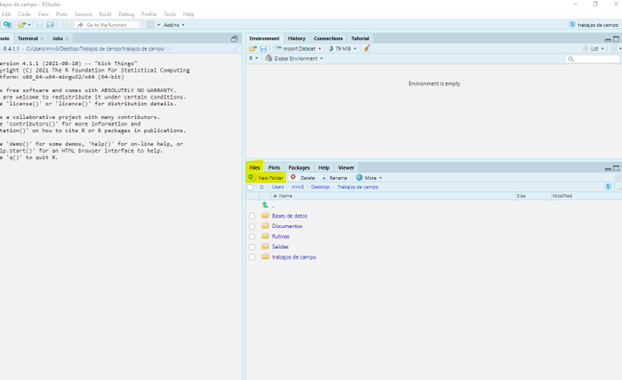
\includegraphics[width=6.19in,height=\textheight,keepaspectratio]{imagenes/01rstudiointerfazinicial.png}

}

\caption{Al finalizar, tu panel de archivos se tendría que ver como se
muestra en la Figura 11}

\end{figure}%

Si has hecho todos estos pasos y tu pantalla se parece a la imagen
anterior es porque has creado un proyecto. Puede verificar el nombre del
proyecto en la esquina superior derecha de la interfaz de RStudio.

Aparte de mantener una organización para mantener todo en orden, la
mayor ventaja de usar proyectos es que a RStudio se le facilita
encontrar dónde están los archivos que serán usados, por ejemplo, si
ubicas las bases de datos correctamente, será más fácil para ti importar
los datos a R y también exportar archivos a otras herramientas de
análisis.

\textbf{\emph{¿Por qué en la imagen anterior falta un panel}}

En la imagen anterior solo vemos 3 ventanas porque no hemos abierto o
creado una rutina, solo tenemos la consola, el panel del ambiente de
trabajo y el panel de archivos.

\section{Archivos de rutina (script) en
R}\label{archivos-de-rutina-script-en-r}

Siguiendo la secuencia de pasos para comenzar a trabajar con R en
Rstudio, vamos a ver uno de los elementos más importantes que son las
rutinas y que la usaremos constantemente.

Hasta este punto, hemos mencionado varias veces la palabra ``rutina''.
Una rutina no es más que un ``documento'' donde escribimos comandos
(funciones, cálculos, etc.), que puede ser ejecutado las veces que sea
necesario (como por ejemplo procesar y generar un reporte semanal).
Realmente crear una rutina es un procedimiento muy sencillo porque se
trata simplemente de escribir en un editor de texto las funciones que
generan los resultados que esperamos.

Dado que podemos salvar las rutinas como archivos, podemos compartirlas
y guardarlas para luego usarlas como referencia.

Para crear una nueva rutina en RStudio vamos a \textbf{\emph{``file''
-\textgreater{} ``new file'' -\textgreater{} ``R Script''}} (en inglés
rutina es igual a \textbf{\emph{Script}} por lo que estaremos utilizando
ambos conceptos de manera indistinta a lo largo del curso).

Después de aceptar ahora tenemos el panel de rutinas habilitado (igual
que un editor de texto) tal como se ilustra en la Figura 12.

Cuando salves la rutina nueva por primera vez, te pedirá dónde guardar
el archivo, entonces procede a guardarlo en la carpeta de ``Rutinas''
que previamente creaste en el Panel de archivos y ya podrás comenzar a
trabajar. Es importante anotar que RStudio no salva el avance de tu
rutina automáticamente, sino que siempre debes guardar cada cierto
tiempo, ya sea a través del menú o utilizando el atajo \textbf{Ctrl+S}.

\begin{figure}[H]

{\centering \pandocbounded{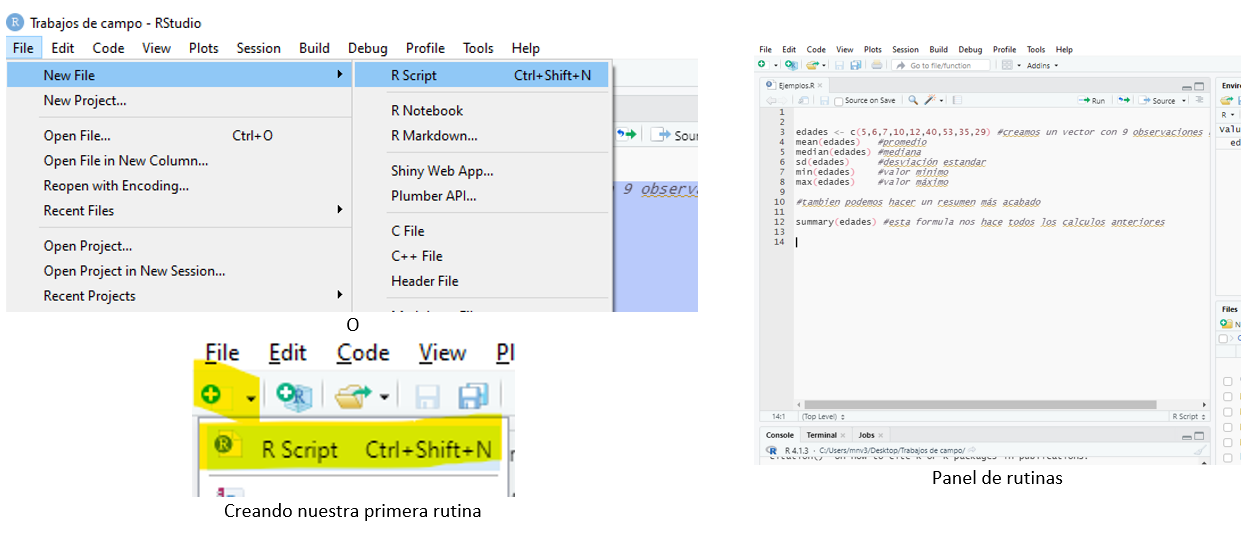
\includegraphics[keepaspectratio]{imagenes/01rutina.png}}

}

\caption{Figura 12. Pasos para comenzar un archivo de rutinas o
(Ctrl+Shift+N)}

\end{figure}%

Si has llegado hasta aquí, entonces ya tienes una gran parte del camino
recorrido, es decir, ya tienes el programa instalado y disponible, un
proyecto creado y tu primera rutina guardada. Si desde ya comenzáramos a
trabajar, podemos escribir comandos directamente en la consola o en el
documento de la rutina para hacer operaciones como aplicar a nuestros
datos los \textbf{estadísticos de tendencia central}, para que vayas
viendo y familiarizándote con R. Vamos a hacer la siguiente prueba paso
a paso:

\begin{enumerate}
\def\labelenumi{\arabic{enumi}.}
\tightlist
\item
  Escribe el texto debajo en el documento de la rutina, o si estas desde
  tu PC, copia y pega todo este texto, selecciónalo (como en cualquier
  editor de texto o Ctrl+A) y presiona \textbf{Ctrl+Enter} o haz clic en
  \textbf{``Run''}.
\end{enumerate}

\begin{Shaded}
\begin{Highlighting}[]
\NormalTok{edades }\OtherTok{\textless{}{-}} \FunctionTok{c}\NormalTok{(}\DecValTok{5}\NormalTok{,}\DecValTok{6}\NormalTok{,}\DecValTok{7}\NormalTok{,}\DecValTok{10}\NormalTok{,}\DecValTok{12}\NormalTok{,}\DecValTok{40}\NormalTok{,}\DecValTok{53}\NormalTok{,}\DecValTok{35}\NormalTok{,}\DecValTok{29}\NormalTok{) }\CommentTok{\#creamos un vector con 9 observaciones numericas }
\FunctionTok{mean}\NormalTok{(edades)   }\CommentTok{\#promedio }
\FunctionTok{median}\NormalTok{(edades) }\CommentTok{\#mediana }
\FunctionTok{sd}\NormalTok{(edades)     }\CommentTok{\#desviación estandar }
\FunctionTok{min}\NormalTok{(edades)    }\CommentTok{\#valor minimo }
\FunctionTok{max}\NormalTok{(edades)    }\CommentTok{\#valor máximo  }
\CommentTok{\#tambien podemos hacer un resumen más acabado, con menos comandos }
\FunctionTok{summary}\NormalTok{(edades) }\CommentTok{\#esta función nos hace todos los calculos anteriores\}}
\end{Highlighting}
\end{Shaded}

\begin{enumerate}
\def\labelenumi{\arabic{enumi}.}
\setcounter{enumi}{1}
\tightlist
\item
  Luego de ejecutar los comandos, podemos ver el resultado en la
  consola. Como puedes observar, está escrito lo mismo que la rutina
  pero debajo de cada comando hay un resultado, es decir, vas a ver el
  resultado de calcular el promedio a través de la función mean() cuyo
  resultado es 21.8, y así sucesivamente. La consoloa debería verse algo
  similar a esto:
\end{enumerate}

\begin{Shaded}
\begin{Highlighting}[]
\NormalTok{edades }\OtherTok{\textless{}{-}} \FunctionTok{c}\NormalTok{(}\DecValTok{5}\NormalTok{,}\DecValTok{6}\NormalTok{,}\DecValTok{7}\NormalTok{,}\DecValTok{10}\NormalTok{,}\DecValTok{12}\NormalTok{,}\DecValTok{40}\NormalTok{,}\DecValTok{53}\NormalTok{,}\DecValTok{35}\NormalTok{,}\DecValTok{29}\NormalTok{) }\CommentTok{\#creamos un vector con 9 observaciones numericas }
\FunctionTok{mean}\NormalTok{(edades)   }\CommentTok{\#promedio }
\end{Highlighting}
\end{Shaded}

\begin{verbatim}
[1] 21.88889
\end{verbatim}

\begin{Shaded}
\begin{Highlighting}[]
\FunctionTok{median}\NormalTok{(edades) }\CommentTok{\#mediana }
\end{Highlighting}
\end{Shaded}

\begin{verbatim}
[1] 12
\end{verbatim}

\begin{Shaded}
\begin{Highlighting}[]
\FunctionTok{sd}\NormalTok{(edades)     }\CommentTok{\#desviación estandar }
\end{Highlighting}
\end{Shaded}

\begin{verbatim}
[1] 17.73728
\end{verbatim}

\begin{Shaded}
\begin{Highlighting}[]
\FunctionTok{min}\NormalTok{(edades)    }\CommentTok{\#valor minimo }
\end{Highlighting}
\end{Shaded}

\begin{verbatim}
[1] 5
\end{verbatim}

\begin{Shaded}
\begin{Highlighting}[]
\FunctionTok{max}\NormalTok{(edades)    }\CommentTok{\#valor máximo  }
\end{Highlighting}
\end{Shaded}

\begin{verbatim}
[1] 53
\end{verbatim}

\begin{Shaded}
\begin{Highlighting}[]
\CommentTok{\#tambien podemos hacer un resumen más acabado, con menos comandos}
\FunctionTok{summary}\NormalTok{(edades) }\CommentTok{\#esta función nos hace todos los calculos anteriores}
\end{Highlighting}
\end{Shaded}

\begin{verbatim}
   Min. 1st Qu.  Median    Mean 3rd Qu.    Max. 
   5.00    7.00   12.00   21.89   35.00   53.00 
\end{verbatim}

Una de las ventajas que tiene RStudio de trabajar con los documentos de
rutina es que puedes tener varias rutinas abiertas a la misma vez y
navegar entre ellas. Esto te puede resultar útil para utilizar una
rutina dentro de otra, es decir, como las rutinas se pueden guardar en
la PC, vas a darte cuenta de que hay muchos procedimientos que se
repiten y que solo necesitas modificarlos levemente, en estos casos,
mientras estás haciendo una rutina puedes usar otra como referencia para
tomar códigos que ya has usado antes o que te han compartido.
\emph{¿Cuál es la ventaja de esto? ¡que no es obligatorio aprenderse
todas las funciones o comandos de R!}

Una muy buena práctica es comentar todo lo que haces para luego saber
qué hiciste en una secuencia de códigos. Para esto, solo tienes que
comenzar una línea con el carácter ``\#'' o signo de número, y todo el
texto después de este carácter cambia de color y se pone en formato
itálico, tornando el texto de color verde de forma predeterminada,
aunque el color verde pudiera variar dependiendo de la configuración de
colores que hayas elegido, tal como te explicamos en la sección 2.2.
Cuando estemos en los pasos de hacer tablas y gráficos, vamos a usar
mucho los comentarios.

El editor de texto de rutina en RStudio también nos permite ver si hay
errores en el código, otra de las tantas funcionalidades que nos ofrece
el programa para hacer más fácil la escritura de códigos.

\begin{figure}[H]

{\centering 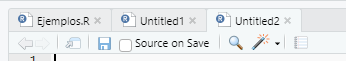
\includegraphics[width=0.5\linewidth,height=\textheight,keepaspectratio]{imagenes/01rutinas2.png}

}

\caption{Varias rutinas abiertas (con \textbf{Ctrl+shift+tab} podemos
movernos entre las rutinas sin usar el ratón)}

\end{figure}%

\bookmarksetup{startatroot}

\chapter{Operadores en R}\label{operadores-en-r}

Antes de seguir debemos conocer algunos conceptos básicos para poder
trabajar con R, y son los operadores como los de comunes de matemáticas
(como suma, división), de asignación, booleanos entre otros. Todos los
lenguaje de programación usan operadores.

Los operadores son los que nos permiten escribir las expresiones que
usaremos en nuestras rutinas y las funciones.

En R hay operadores que se usan muy constantemente para crear nuestro
código, R desde que se tiene abierto puede servir como una calculadora
(muy avanzada, por cierto), es decir, si escribes en la consola 2+2 y
presionas \textbf{Enter} tendrás un resultado, pero si queremos correr
varias veces esta misma operación podemos guardarla en un
\textbf{objeto} y en vez de escribir de nuevo la operación (el 2+2)
podemos simplemente llamar este \textbf{objeto} con solo escribirlo y
vamos a obtener el mismo resultado. manejar los objetos nos agiliza
mucho el trabajo.

Dentro de las funciones podemos ver si un valor está presente o un
objeto, así como también reasignar un valor o proceder hacer operaciones
matemáticas.

\subsection{\texorpdfstring{\textbf{Resumen de los operadores más usados
para la escritura de las expresiones en
R}}{Resumen de los operadores más usados para la escritura de las expresiones en R}}\label{resumen-de-los-operadores-muxe1s-usados-para-la-escritura-de-las-expresiones-en-r}

\begin{longtable}[]{@{}
  >{\raggedright\arraybackslash}p{(\linewidth - 6\tabcolsep) * \real{0.0223}}
  >{\raggedright\arraybackslash}p{(\linewidth - 6\tabcolsep) * \real{0.0318}}
  >{\raggedright\arraybackslash}p{(\linewidth - 6\tabcolsep) * \real{0.4793}}
  >{\raggedright\arraybackslash}p{(\linewidth - 6\tabcolsep) * \real{0.4634}}@{}}
\toprule\noalign{}
\begin{minipage}[b]{\linewidth}\raggedright
Tipo
\end{minipage} & \begin{minipage}[b]{\linewidth}\raggedright
Operador
\end{minipage} & \begin{minipage}[b]{\linewidth}\raggedright
Descripción
\end{minipage} & \begin{minipage}[b]{\linewidth}\raggedright
Ejemplo
\end{minipage} \\
\midrule\noalign{}
\endhead
\bottomrule\noalign{}
\endlastfoot
Asignación & \textless- & Para asignar un valor a un objeto (el signo de
= es similar) se compone de ``menor que'' seguido de una raya o ``dash''
& x \textless- 2+2 con esto creamos (asignamos) la operación 2+2 al
objeto x

si volvemos a usar x como objeto y le asignamos otro valor, este se
sobrescribirá \\
Asignación & '' '' & Las comillas son para declarar texto, si escribes
cualquier caracter entre comillas será reconocida como una cadena de
caracteres & z~ \textless- ``Me gusta R'' asignamos al objeto z el
texto \\
Evaluación & == & igual, igual significa Igual, para evaluar si un
objeto es igual a otro o una variable es igual a un valor & x ==4 (la
respuesta es TRUE) \\
Evaluación & != & Significa no es igual, para evaluar si un objeto es
diferente a otro o una variable es diferente a un valor. & x != 4 (la
respuesta es FALSE) \\
Evaluación & \textgreater, \textless, \textgreater=, \textless= & Signos
para evaluar mayor que, menor que, mayor o igual que y menor o igual
que, aparte de los números, estos operadores funcionan con texto, (b es
menor que c por ejemplo) & x\textless5 (la respuesta es TRUE),
x\textgreater5 (la respuesta es FALSE)

x\textgreater=3 (la respuesta es TRUE)

x\textless=5 (la respuesta es FALSE) \\
Evaluación & \%in\% & Identifica si un elemento (como un número, por
ejemplo) está dentro de un objeto (si queremos decir ``no esta incluido
en'' solo agregamos signo de exclamación !) & 2 \%in\% x (la respuesta
es TRUE)

2 !\%in\% x (la respuesta es FALSE) \\
Acceso & \$ & Signo de dinero sirve para acceder a las variables de un
dataframe o una lista & mtcars (un dataframe interno de R) tiene 11
columnas, para seleccionar o aplicar una función a una de estas (como
\textbf{mean} para promedio) escribes el nombre del dataframe seguido
del signo de dinero y el nombre de la variable así :
\textbf{mean(mtcars\$cyl)} para retornar el promedio o 6.1875 \\
Acceso & {[} {]} & Los corchetes son usados con los vectores, matrices y
dataframe para acceder a un valor en base de una posición (para las
matrices y dataframe) donde el primer valor es el numero de fila y el
segundo valor es el numero de columna. Para los vectores solo se usa un
valor para especificar la posción. & usando \textbf{mtcars} de nuevo, si
quiero saber que valor está en la fila 20 de la columna 3 puedes
escribir este código \textbf{mtcars{[}20,3{]}} y retorna 71.1 que es el
valor de la variable \textbf{disp} de la fila del carro toyota
corolla. \\
Booleano & \& & Y o AND & \textbf{y} = c(1,3,4,9,11,10) \#un vector con
6 elementos

3 \& 4 \%in\% y (la respuesta es TRUE, porque están ambos, si no es así,
es FALSE ) \\
Booleano & \textbar{} & O o OR & 3 \textbar{} 30 \%in\% y (la respuesta
es TRUE, porque está al menos 1 de los elementos dentro del objeto o
vector \textbf{y}, si ambos elementos faltaran, la respuesta seria
FALSE) \\
Aritméticos & +, -, *, /,\^{}, = & Signos matemáticos para suma, resta,
multiplicación, división y exponente. El igual es usado más para
asignación & 2*2 retorna 4

2+2 retorna 4

4/2 retorna 2

x = 2+2 (igual como asignación, otro ejemplo x\textbf{=}log(4),donde
log() es una función que la usamos para asignar al objeto x el logaritmo
de 4) \\
Otros & ( ) & Los paréntesis son símbolos que se usan mucho en
operaciones y funciones para determinar que ocurra algo y en el orden,
siempre desde los más internos hacia los externos & mean(c(3,4,5,6,2,5))
el resultado es 4.16, si te fijas primero tenemos un set de paréntesis
que crea un objeto, luego el otro set de paréntesis que indica calcular
el promedio de este grupo usando la función \textbf{\emph{mean(),}} \\
Otros & \%\textgreater\% o ``pipe'' & Es un operador para indicar una
secuencia de comandos o expresiones que se realizan a partir de un
objeto en cascada, significa ``entonces o luego'' (vamos a ver más de su
uso cuando veamos transformación de datos) se puede escribir con Ctrl+M
y hay que tener instalado el paquete \textbf{tidyverse} &
c(3,4,5,6,2,5)\%\textgreater\%

mean() nos da el mismo resultado que

mean(c(3,4,5,6,2,5)), básicamente una expresión como esta nos dice
``crea un objeto de 5 numeros, \textbf{Entonces} (el pipe) obtén el
promedio'' \\
otros & , (comma) & La coma en R se usa para asignar un espacio de un
elemento o un parámetro, por ejemplo, el primer elemento luego una coma,
segundo elemento y luego una coma & y \textless- c(``a''\textbf{,}
``b''\textbf{,}''c'')

ggplot(data=df, aes(x=var1\textbf{,} y=var2\textbf{,} fill=cat1)) \\
\end{longtable}

A medida que vayas practicando los operadores se van haciendo familiares
y más fácil de entender. Siempre hay que tomar en cuenta que un operador
mal usado dará error cuando ejecutamos un comando o código (es muy común
dejar de escribir el último paréntesis, o cerrar comillas).

\bookmarksetup{startatroot}

\chapter{Objetos en R}\label{objetos-en-r}

Otro elemento de suma importancia a conocer cuando se trabaja con R (así
como vimos la importancia de las rutinas) son los objetos y sus
diferentes tipos, dado que es con esto que trabajamos, son básicamente
los contenedores de los datos (que R los almacena en la memoria del
computador) es decir, a partir de estos es que haremos nuestras salidas
como tablas, gráficos, reportes a través de la transformación (declarar,
nombrar, filtrar reemplazar). Básicamente los objetos son el fundamento
de todo.

~En R hay 5 tipos de objetos de datos y se dividen en dos grupos de
objetos, los que son de un solo tipo de dato (atómicos) o los que tienen
varios tipos de datos (recursivos)

\section{Vectores}\label{vectores}

Dentro de los objetos atómicos tenemos \textbf{los vectores}, que no
tienen dimensión, es decir, filas o columnas y pueden ser de clase
numérico (entero y decinal), integer (números enteros solamente),
carácter o texto, lógico (TRUE, FALSE) y factor (jerarquía en los
valores). Un ejemplo de creación de un vector es el siguiente:

\pandocbounded{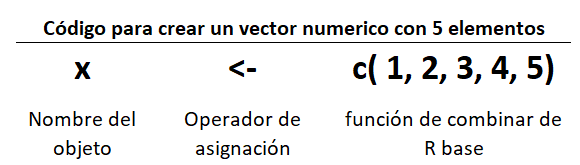
\includegraphics[keepaspectratio]{imagenes/05vector.png}}

\pandocbounded{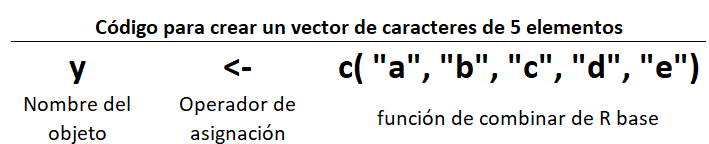
\includegraphics[keepaspectratio]{imagenes/05vector2.png}}

Para los vectores que son de caracteres o texto cuando los creamos si
ponemos números sin comillas, estos cuando lo llamemos serán reconocidos
como texto, por lo tanto no se pueden hacer operaciones matemáticas con
estos aunque tengan números.

Si escribes ``x'' (o el nombre que hayas usado para crear el vector) y
presionas \textbf{Enter,} en la consola observaras los elementos
contenidos en este vector.

Una de las funcionalidades más interesantes de R es que por ejemplo en
el caso de vectores numéricos, si haces una operación matemática,
ejemplo 5 + \textbf{x} (nombre del vector), la operación se hará en
todos los elementos del vector, es decir, el 5 se sumara con cada uno de
los números. Si haces esto con un vector de texto o carácter, en la
consola observaras un error que es una operación entre un argumento no
numérico contra otro numérico.

A medida que avancemos con el desarrollo de los productos vamos a ver
que los vectores los usamos de forma constante, un ejemplo común es
crear un vector con los nombres de las provincias o municipios de
interés para luego cuando vamos a filtrar la base con la que estamos
trabajando podemos hacer este filtro invocamos el dicho vector. También
combinando varios tipos de vectores, con las mismas dimensiones, es
decir el mismo numero de elementos podemos ``unirlos'' y formar un nuevo
objeto como un \textbf{dataframe} o una lista.

\section{Matrices}\label{matrices}

Otro tipo de objeto atómico o que solo admite un tipo de valor es
\textbf{la matriz} que es básicamente un vector pero con dos dimensiones
(columnas y filas) se crean usando la función \textbf{matrix()} y se le
debe agregar el parámetro del total de filas así como el total de
columnas por ejemplo de la siguiente forma:

\pandocbounded{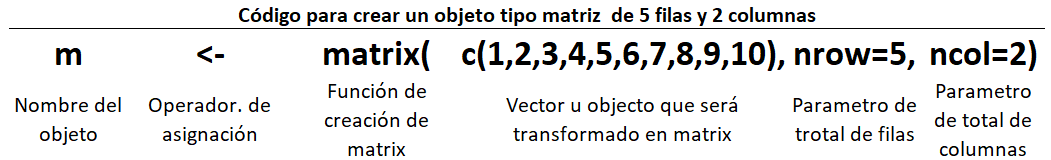
\includegraphics[keepaspectratio]{imagenes/05matrix.png}}

No entraré mucho en detalle con los objetos de tipo matriz porque estos
objetos tienen sus usos bien específicos y no vamos a usarlos de forma
constante como los vectores.

\section{Dataframes}\label{dataframes}

Ahora vamos a ver uno de los objetos más importantes que vamos a usar
que son los \textbf{dataframes}, que es un objeto de tipo recursivo o
que admite varios tipos de datos (texto, numérico, lógico) y es idéntico
a una tabla, es decir, tiene dos dimensiones, columnas y filas. Las
columnas se pueden ver como si fueran variables y las filas son los
valores contenidos en esta variable.

Para los trabajos que vamos a realizar, este será el tipo de objeto
quizás más nos sentiremos familiarizados dado que lo más parecido a un
dataframe es una base de datos, ya sea en Excel u otro tipo de programa.

Una de las ventajas que tiene Rstudio es que nos ayuda a fácilmente ver
la estructura del objeto dataframe, (cuantas variables o columnas y
cuantas filas u observaciones) también para visualizar el contenido.

\begin{figure}[H]

{\centering \pandocbounded{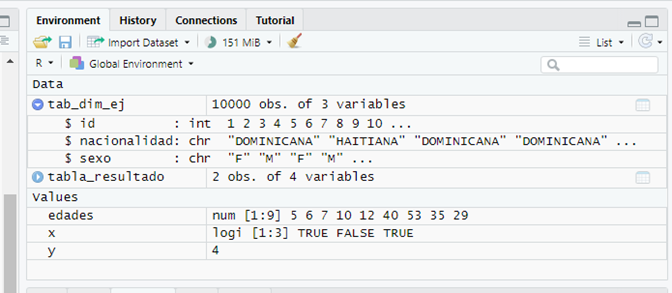
\includegraphics[keepaspectratio]{imagenes/05dataframe.png}}

}

\caption{Panel de ambiente de trabajo en Rstudio donde podemos ver los
objetos de datos disponibles, en esta imagen podemos ver dos dataframes
(tab\_dim\_ej y tabla\_resultado) y debajo, en la categoría de values, 3
vectores, (edades, x y ``y'') . Rstudio nos permite diferencial
rápidamente también ver los atributos de cada elemento. Para saber más
sobre los tipos de objetos podemos usar dos funciones str() y class(),
la primera para ver la estructura y la segunda para ver que clase de
objeto es.}

\end{figure}%

Para comenzar a usar los \textbf{dataframes} tenemos dos formas de
hacerlo, primero es creándolo directamente, es decir, a través de
escribir los datos que usaremos combinando varios vectores como el
siguiente ejemplo, para crear una pequeña base de datos o tabla:

\begin{Shaded}
\begin{Highlighting}[]
\NormalTok{ var1 }\OtherTok{\textless{}{-}} \FunctionTok{c}\NormalTok{(}\StringTok{"maria"}\NormalTok{, }\StringTok{"pedro"}\NormalTok{, }\StringTok{"juan"}\NormalTok{, }\StringTok{"jose"}\NormalTok{) }\CommentTok{\#creamos un vector con nombres por ejemplo}
\NormalTok{ var2 }\OtherTok{\textless{}{-}} \FunctionTok{c}\NormalTok{(}\DecValTok{25}\NormalTok{, }\DecValTok{40}\NormalTok{, }\DecValTok{30}\NormalTok{, }\DecValTok{35}\NormalTok{) }\CommentTok{\#creamos otro vector con las edades}
\NormalTok{ var3 }\OtherTok{\textless{}{-}} \FunctionTok{c}\NormalTok{(}\StringTok{"F"}\NormalTok{, }\StringTok{"M"}\NormalTok{, }\StringTok{"M"}\NormalTok{, }\StringTok{"M"}\NormalTok{) }\CommentTok{\#creamos otro vector con el sexo}
\NormalTok{ var4 }\OtherTok{\textless{}{-}} \FunctionTok{c}\NormalTok{(}\StringTok{"LR"}\NormalTok{, }\StringTok{"SD"}\NormalTok{, }\StringTok{"SC"}\NormalTok{, }\StringTok{"PP"}\NormalTok{) }\CommentTok{\# creamos otro vector con la procedencia}
\NormalTok{ tabla }\OtherTok{\textless{}{-}} \FunctionTok{data.frame}\NormalTok{(}\AttributeTok{nombre=}\NormalTok{var1, }\AttributeTok{edad=}\NormalTok{var2, }\AttributeTok{sexo=}\NormalTok{var3, }\AttributeTok{prov=}\NormalTok{var4)}
 
\NormalTok{tabla}
\end{Highlighting}
\end{Shaded}

\begin{verbatim}
  nombre edad sexo prov
1  maria   25    F   LR
2  pedro   40    M   SD
3   juan   30    M   SC
4   jose   35    M   PP
\end{verbatim}

\begin{figure}[H]

{\centering \pandocbounded{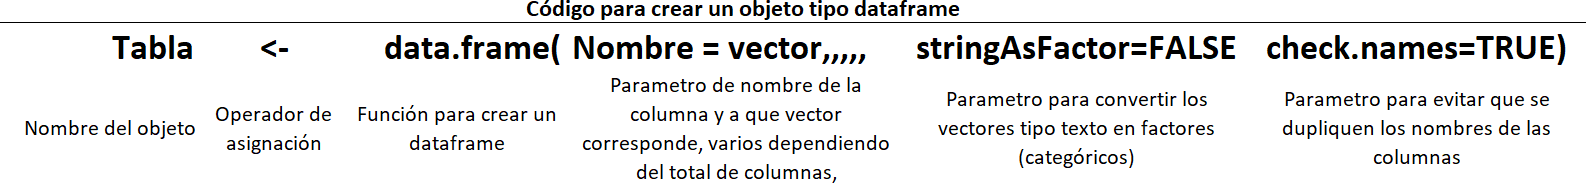
\includegraphics[keepaspectratio]{imagenes/05dataframe2.png}}

}

\caption{Anatomía de la función data.frame() para crear un dataframe. en
R las funciones vienen con valores en los parámetros de forma
predeterminada, incluso no hay que escribirlos. Un ejemplo es en esta
función de \textbf{data.frame()} el parámetro
\textbf{\emph{check.names=TRUE}} viene predeterminado y por ende no hay
que escribirlo.}

\end{figure}%

Entonces si corremos las líneas anteriores vamos a tener como resultado
un dataframe nuevo con 4 variables y 4 observaciones, \textbf{Ojo}, los
vectores deben de tener la misma cantidad de elementos o sino vemos el
siguiente error, \textbf{\emph{``Error in data.frame(nombre = var1, edad
= var2, sexo = var3, prov = var4) :~ arguments imply differing number of
rows: 4, 3''}}que significa que uno de los vectores no tiene la misma
cantidad de elementos.

Para corregir esto, si el valor es desconocido en el vector que nos
falta un elemento, solo agregamos un elemento nuevo llamado
\textbf{\emph{NA,}} sin comillas, que es una forma de decirle a R que el
valor es desconocido y corremos de nuevo las líneas donde hicimos el
cambio para actualizar.

Este abordaje puede ser útil para tablas pequeñas, pero cuando tenemos
que trabajar con bases de datos que tienen cientos o miles de
observaciones entonces creamos un dataframe importando los datos desde
diferentes fuentes, como archivos de Excel, desde archivos de texto,
incluso archivos nativos de otros programas de estadísticas como SPSS o
STATA.

En Rstudio podemos sin necesidad de escribir una expresión o comando
usando el botón de ``\textbf{import Dataset''} en el panel de ambiente
de trabajo y al hacer clic se nos despliega un menú para diferentes
tipos de formatos de bases de datos como Excel, csv o txt, SPSS, SAS,
Stata.

\begin{figure}[H]

{\centering \pandocbounded{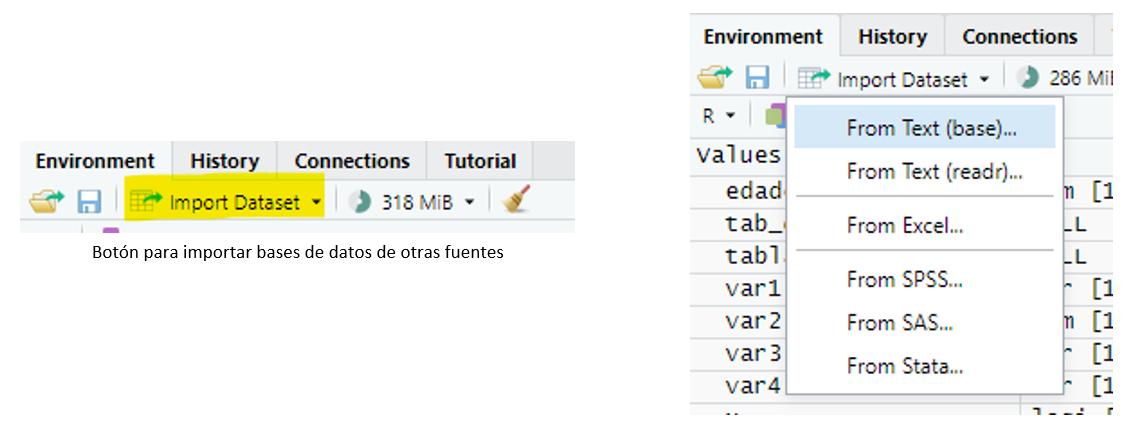
\includegraphics[keepaspectratio]{imagenes/05importdatagrame.png}}

}

\caption{Botón para importar bases de datos de otras fuentes}

\end{figure}%

Después de hacer clic en uno de los formatos, (ejemplo Excel) se abre
una ventana para seleccionar el archivo de la base de datos, que
variables o columnas vamos a incluir además de otros parámetros.

\begin{figure}[H]

{\centering \pandocbounded{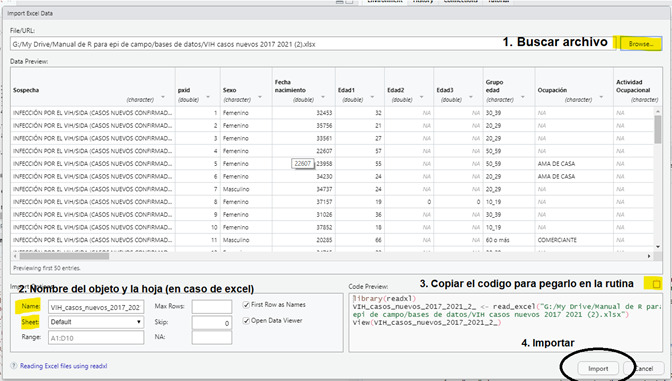
\includegraphics[keepaspectratio]{imagenes/05importdatagrame2.png}}

}

\caption{Pasos para importar un dataframe usando Rstudio}

\end{figure}%

Por ejemplo de forma predeterminada en el nombre del objeto o dataframe
estará el nombre del archivo de la base de datos, puedes cambiarlo a un
nombre más amigable (ejemplo bd o base) también si estás usando una base
de Excel y esta contiene varias hojas, puedes especificar cual hoja
usaras en \textbf{``sheet''}, incluso el rango, es decir, si solo usaras
hasta ciertas filas, también puedes poner desde que fila se leerá el
archivo, a veces en las bases de datos de Excel se les coloca títulos y
los datos se comienzan a digitar a partir de la 3ra o 4ta fila entonces
puedes en \textbf{``skip''} omitir la filas que no son necesaria.

Por último, si este proceso lo vas a usar repetidamente, debes copiar el
código que está en el campo inferior derecho de la ventana y pegarlo en
el panel de editor de rutinas para que lo tengas en tu rutina. Incluso
luego de que lo tengas ya en tu rutina, puedes modificarlo de ser
necesario (realmente este es un aditamento visual dado que Rstudio está
generando un código para que no tengas que escribirlo, básicamente
Rstudio está cargando el paquete readxl, luego usando la función de
importar archivos de Excel llamada \textbf{read\_excel()}.

Otra forma para cargar bases de datos muy parecido a lo que vimos
anteriormente es usando el paquete \textbf{rio (input/output)} y el
paquete \textbf{here} usando la función \textbf{import()} en combinación
y la función \textbf{here()} (que nos ahorra escribir toda la ruta del
archivo de la base de datos cuando estamos en un proyecto en Rstudio) ,
aquí un ejemplo:

La base que voy a importar está ubicada en la carpeta de Base de datos,
solo necesito saber el nombre del archivo que voy a usar, en este caso
``base de dato se de datos ejemplo.xlsx''

\begin{Shaded}
\begin{Highlighting}[]
\NormalTok{mi\_base\_ejemplo }\OtherTok{\textless{}{-}} \FunctionTok{import}\NormalTok{(}\FunctionTok{here}\NormalTok{(}\StringTok{"Bases de datos"}\NormalTok{, }\StringTok{"base de datos ejemplo.xlsx"}\NormalTok{), }\AttributeTok{setclass=}\NormalTok{”tibble”)}
\end{Highlighting}
\end{Shaded}

Luego podemos ver la base con la función \textbf{View()} para invocar el
visor de datos o simplemente \textbf{head()} para ver las primeras
observaciones del dataframe en la consola. Como buena práctica, después
de importar la base de datos en un dataframe es ver su estructura para
determinar si las columnas se importaron bien, podemos hacerlo viendo en
el panel de ambiente de trabajo desplegando la flecha a la izquierda del
nombre del dataframe o escribiendo en la consola la función
\textbf{str()} donde vamos a ver el nombre de la variable, de que clase
es (chr si es texto, num si es numérico, logi si es lógico (true/false ,
int si es interger), factor, etc..

Si vemos por ejemplo que una variable que sabemos de antemano que es una
fecha está como tipo numérica, luego podemos transformarla a su tipo
original. Más adelante veremos cómo se hace.

\begin{longtable}[]{@{}
  >{\raggedright\arraybackslash}p{(\linewidth - 2\tabcolsep) * \real{0.2018}}
  >{\raggedright\arraybackslash}p{(\linewidth - 2\tabcolsep) * \real{0.7982}}@{}}
\caption{\textbf{Funciones que nos sirven para revisar un dataframe
(solo debemos poner el nombre del dataframe dentro de los
paréntesis)}}\tabularnewline
\toprule\noalign{}
\begin{minipage}[b]{\linewidth}\raggedright
Función
\end{minipage} & \begin{minipage}[b]{\linewidth}\raggedright
Efecto
\end{minipage} \\
\midrule\noalign{}
\endfirsthead
\toprule\noalign{}
\begin{minipage}[b]{\linewidth}\raggedright
Función
\end{minipage} & \begin{minipage}[b]{\linewidth}\raggedright
Efecto
\end{minipage} \\
\midrule\noalign{}
\endhead
\bottomrule\noalign{}
\endlastfoot
head() & Muestra las 6 primeras filas \\
tail() & Muestra las ultimas 6 filas \\
dim() & Nos muestra las dimensiones del dataframe, total de
observaciones y total de columnas \\
nrow() & Nos muestra el total de filas u observaciones \\
ncol() & Nos muestra el total de columnas \\
str() & Nos hace un resumen de la estructura del dataframe, columna por
columna \\
names() o colnames() & Nos muestra los nombres de las columnas \\
\end{longtable}

Los resultados que arrojan estas funciones podemos guardarlas en un
objeto (ej.vector) por ejemplo si queremos comparar el total de columna
de un dataframe vs otro (por ejemplo un corte de la base de datos de una
fecha vs otro corte) podemos crear el vector col\_dataframe\_1
\textless- ncol(dataframe1) y el vector col\_dataframe\_2 \textless-
ncol(dataframe2) y luego comparar: col\_dataframe1 ==col\_dataframe2, si
tenemos el resultado TRUE, pues ambos dataframes tienen la misma
cantidad de columnas, de lo contrario, uno de los dataframes tiene de
menos o de más columnas.

Por igual se hacemos el mismo ejercicio para ver cuantas filas ha
crecido una base de datos podemos usar la función nrow() y restar el
vector del dataframe2 -- dataframe1 para obtener la diferencias de
filas.

Esto es un ejemplo muy sencillo pero muchos procedimientos de
transformación de datos usamos estas funciones.

\section{Listas}\label{listas}

Otro tipo de objeto que usa R son las listas, que es un tipo de objeto
recursivo o que admite diferentes formatos de elementos. Las listas
básicamente son objetos que combinan varios objetos que pueden ser
matrices, vectores, dataframes sin restricciones. En resumen, las listas
son mini contenedores, se usan mucho para las funciones cuando
necesitamos ``pegar'' o usar objetos de diferentes formatos para obtener
un solo resultado. También cuando hacemos \textbf{``for loops''} o
bucles (una forma de hacer tareas repetitivas) se usan mucho las listas.
El manejo de listas es un poco avanzado para comenzar a trabajar en R,
pero son muy importantes.

Cuando tratamos de visualizar una lista el resultado que vemos en la
consola son primero el orden del objeto dentro de doble corchete y luego
el contenido del objeto, así (copia y pega en la consola el siguiente
texto):

\begin{Shaded}
\begin{Highlighting}[]
\CommentTok{\#vamos a crear varios objetos }

\NormalTok{vect1 }\OtherTok{\textless{}{-}} \FunctionTok{c}\NormalTok{(}\StringTok{"a"}\NormalTok{, }\StringTok{"b"}\NormalTok{, }\StringTok{"c"}\NormalTok{)}
\NormalTok{vect2 }\OtherTok{\textless{}{-}} \FunctionTok{c}\NormalTok{(}\FunctionTok{seq}\NormalTok{(}\DecValTok{1}\SpecialCharTok{:}\DecValTok{10}\NormalTok{))}
\NormalTok{vect3 }\OtherTok{\textless{}{-}}\NormalTok{ letters}
\NormalTok{vect4 }\OtherTok{\textless{}{-}}\NormalTok{ mtcars[}\DecValTok{1}\SpecialCharTok{:}\DecValTok{5}\NormalTok{,}\DecValTok{2}\SpecialCharTok{:}\DecValTok{3}\NormalTok{]}
\CommentTok{\#vamos a crear una lista de objetos}

\NormalTok{lista }\OtherTok{\textless{}{-}} \FunctionTok{list}\NormalTok{(vect1, vect2, vect3, vect4)}
\end{Highlighting}
\end{Shaded}

Si desde la misma consola llamamos al objeto lista que creamos (solo
escribiendo el nombre del objeto, ``lista'' en este caso tendremos el
siguiente resultado:

\begin{Shaded}
\begin{Highlighting}[]
\NormalTok{lista}
\end{Highlighting}
\end{Shaded}

\begin{verbatim}
[[1]]
[1] "a" "b" "c"

[[2]]
 [1]  1  2  3  4  5  6  7  8  9 10

[[3]]
 [1] "a" "b" "c" "d" "e" "f" "g" "h" "i" "j" "k" "l" "m" "n" "o" "p" "q" "r" "s"
[20] "t" "u" "v" "w" "x" "y" "z"

[[4]]
                  cyl disp
Mazda RX4           6  160
Mazda RX4 Wag       6  160
Datsun 710          4  108
Hornet 4 Drive      6  258
Hornet Sportabout   8  360
\end{verbatim}

También desde el panel del ambiente de trabajo en Rstudio podemos ver
los objetos tipo listas, cuantos elementos tiene y si desplegamos
podemos ver sus elementos, así como también el tipo de elemento y
características.

\begin{figure}[H]

{\centering \pandocbounded{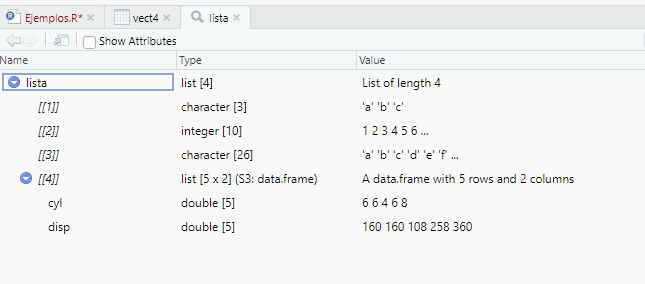
\includegraphics[keepaspectratio]{imagenes/05listas.png}}

}

\caption{Si queremos llamar un objeto dentro de una lista simplemente
escribimos el nombre de la lista abrimos doble corchete y ponemos dentro
el numero de orden que corresponde el elemento que queremos,}

\end{figure}%

\begin{Shaded}
\begin{Highlighting}[]
\NormalTok{lista[[}\DecValTok{1}\NormalTok{]] }\CommentTok{\#nos nos arroja el resultado de todo el contenido del elemento 1, que en este caso es un vector}
\end{Highlighting}
\end{Shaded}

\begin{verbatim}
[1] "a" "b" "c"
\end{verbatim}

Dentro de los ejercicios que vamos a hacer usaremos las listas, por
ejemplo, con estas podemos cargar múltiples archivos como objetos desde
una carpeta para facilitar el proceso de importación.

\section{Funciones}\label{funciones}

Otro tipo de objeto que no necesariamente almacena datos pero a través
de esto si creamos objetos de datos son las funciones y si te has dado
cuenta hasta ahora se han mencionado mucho dado que todo el código que
vamos a ir escribiendo mayormente se hace con funciones, de hecho, como
se mencionó arriba, la mayoría de los paquetes son una compilación de
funciones. Nosotros podemos crear funciones que usan funciones ya sean
de R base o incluso de otros paquetes.

Las funciones nos ayudan a agilizar el trabajo dado que son un set de
instrucciones dentro de nuestra rutina. Un ejemplo podemos crear una
función que nos produzca un gráfico de curva epidémica de un periodo y
un lugar determinados (tenemos un resultado, el gráfico, y dos
parámetros, el periodo y el lugar).

Para crear una función usamos la siguiente sintaxis:

\pandocbounded{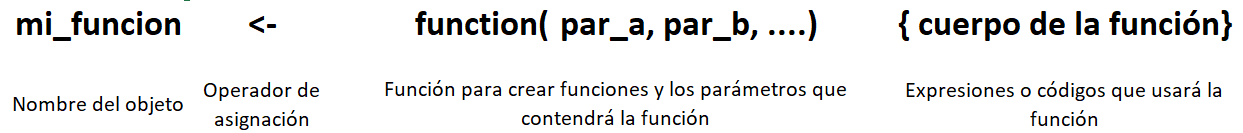
\includegraphics[keepaspectratio]{imagenes/05funcion.png}}

Vamos hacer un ejercicio simple para entender mejor una función:

\begin{Shaded}
\begin{Highlighting}[]
\CommentTok{\#una funcion para calcular el indice de masa corporal}
\NormalTok{mi\_funcion }\OtherTok{\textless{}{-}} \ControlFlowTok{function}\NormalTok{(peso, altura)\{ }
  
\NormalTok{  resultado }\OtherTok{\textless{}{-}} \FunctionTok{round}\NormalTok{(peso}\SpecialCharTok{/}\NormalTok{(altura}\SpecialCharTok{/}\DecValTok{100}\NormalTok{)}\SpecialCharTok{\^{}}\DecValTok{2}\NormalTok{,}\DecValTok{2}\NormalTok{) }\CommentTok{\#asigna al elemento resultado el la operación entre peso y altura y luego redondear el valor}
  
  \FunctionTok{print}\NormalTok{(}\FunctionTok{paste0}\NormalTok{(}\StringTok{"Formula: "}\NormalTok{,peso,}\StringTok{"kg./"}\NormalTok{,altura}\SpecialCharTok{/}\DecValTok{100}\NormalTok{,}\StringTok{"(m)2"}\NormalTok{)) }\CommentTok{\# retorna un texto con el peso y la altura}
  
  \FunctionTok{print}\NormalTok{(}\FunctionTok{paste0}\NormalTok{(}\StringTok{"El indice de masa corporal es "}\NormalTok{, resultado)) }\CommentTok{\# retorna el en un solo texto el indice de masa corporal obtenido}
  
\NormalTok{\}}

\FunctionTok{mi\_funcion}\NormalTok{(}\AttributeTok{peso=}\DecValTok{115}\NormalTok{,}\AttributeTok{altura=}\DecValTok{180}\NormalTok{) }\CommentTok{\#llamamos la funcion y escribimos los parametros}
\end{Highlighting}
\end{Shaded}

\begin{verbatim}
[1] "Formula: 115kg./1.8(m)2"
[1] "El indice de masa corporal es 35.49"
\end{verbatim}

Entonces, para entender mejor como trabaja una función, usando el
ejemplo anterior, luego del nombre de la función y el operador de
asignación, escribimos la función function()\{ \} y dentro de los
paréntesis escribimos el nombre que queramos usar para los parámetros,
separados por comma (como hicimos en el ejemplo anterior, usamos peso y
altura) luego dentro de las llaves vamos a proceder a escribir las
expresiones para obtener un resultado, para esta función del cálculo del
índice de masa corporal creamos un vector que es el resultado de la
operación de la fórmula del IMC, donde el parámetro 1, el peso es
dividido entre el parámetro 2, la altura que a su vez es dividida entre
100 y luego elevada al cuadrado, después la siguiente expresión presenta
un texto con los parámetros y luego presenta otro texto con el resultado
del IMC.\\
De las funciones se pueden escribir libros, hay una vasta documentación
de como trabajar con ellas, básicamente son el pilar para lo que es la
programación en R.

Mi gran sugerencia es cuando te sientas más familiarizado y tengas más
experiencia en R, puedes dedicarle tiempo a aprender sobre como trabajar
más profundamente con las funciones. Por ahora vamos a enfocarnos en los
paquetes que tienen funciones que nos facilitan el trabajo para análisis
de datos.

\bookmarksetup{startatroot}

\chapter*{References}\label{references}
\addcontentsline{toc}{chapter}{References}

\markboth{References}{References}

\phantomsection\label{refs}
\begin{CSLReferences}{0}{1}
\end{CSLReferences}




\end{document}
